\documentclass[]{article}
\usepackage[T1]{fontenc}
\usepackage{lmodern}
\usepackage{amssymb,amsmath}
\usepackage{ifxetex,ifluatex}
\usepackage{fixltx2e} % provides \textsubscript
% use upquote if available, for straight quotes in verbatim environments
\IfFileExists{upquote.sty}{\usepackage{upquote}}{}
\ifnum 0\ifxetex 1\fi\ifluatex 1\fi=0 % if pdftex
  \usepackage[utf8]{inputenc}
\else % if luatex or xelatex
  \ifxetex
    \usepackage{mathspec}
    \usepackage{xltxtra,xunicode}
  \else
    \usepackage{fontspec}
  \fi
  \defaultfontfeatures{Mapping=tex-text,Scale=MatchLowercase}
  \newcommand{\euro}{€}
\fi
% use microtype if available
\IfFileExists{microtype.sty}{\usepackage{microtype}}{}
\usepackage{color}
\usepackage{fancyvrb}
\newcommand{\VerbBar}{|}
\newcommand{\VERB}{\Verb[commandchars=\\\{\}]}
\DefineVerbatimEnvironment{Highlighting}{Verbatim}{commandchars=\\\{\}}
% Add ',fontsize=\small' for more characters per line
\newenvironment{Shaded}{}{}
\newcommand{\KeywordTok}[1]{\textcolor[rgb]{0.00,0.44,0.13}{\textbf{{#1}}}}
\newcommand{\DataTypeTok}[1]{\textcolor[rgb]{0.56,0.13,0.00}{{#1}}}
\newcommand{\DecValTok}[1]{\textcolor[rgb]{0.25,0.63,0.44}{{#1}}}
\newcommand{\BaseNTok}[1]{\textcolor[rgb]{0.25,0.63,0.44}{{#1}}}
\newcommand{\FloatTok}[1]{\textcolor[rgb]{0.25,0.63,0.44}{{#1}}}
\newcommand{\CharTok}[1]{\textcolor[rgb]{0.25,0.44,0.63}{{#1}}}
\newcommand{\StringTok}[1]{\textcolor[rgb]{0.25,0.44,0.63}{{#1}}}
\newcommand{\CommentTok}[1]{\textcolor[rgb]{0.38,0.63,0.69}{\textit{{#1}}}}
\newcommand{\OtherTok}[1]{\textcolor[rgb]{0.00,0.44,0.13}{{#1}}}
\newcommand{\AlertTok}[1]{\textcolor[rgb]{1.00,0.00,0.00}{\textbf{{#1}}}}
\newcommand{\FunctionTok}[1]{\textcolor[rgb]{0.02,0.16,0.49}{{#1}}}
\newcommand{\RegionMarkerTok}[1]{{#1}}
\newcommand{\ErrorTok}[1]{\textcolor[rgb]{1.00,0.00,0.00}{\textbf{{#1}}}}
\newcommand{\NormalTok}[1]{{#1}}
\usepackage{longtable,booktabs}
\usepackage{graphicx}
% Redefine \includegraphics so that, unless explicit options are
% given, the image width will not exceed the width of the page.
% Images get their normal width if they fit onto the page, but
% are scaled down if they would overflow the margins.
\makeatletter
\def\ScaleIfNeeded{%
  \ifdim\Gin@nat@width>\linewidth
    \linewidth
  \else
    \Gin@nat@width
  \fi
}
\makeatother
\let\Oldincludegraphics\includegraphics
{%
 \catcode`\@=11\relax%
 \gdef\includegraphics{\@ifnextchar[{\Oldincludegraphics}{\Oldincludegraphics[width=\ScaleIfNeeded]}}%
}%
\ifxetex
  \usepackage[setpagesize=false, % page size defined by xetex
              unicode=false, % unicode breaks when used with xetex
              xetex]{hyperref}
\else
  \usepackage[unicode=true]{hyperref}
\fi
\hypersetup{breaklinks=true,
            bookmarks=true,
            pdfauthor={},
            pdftitle={},
            colorlinks=true,
            citecolor=blue,
            urlcolor=blue,
            linkcolor=magenta,
            pdfborder={0 0 0}}
\urlstyle{same}  % don't use monospace font for urls
\setlength{\parindent}{0pt}
\setlength{\parskip}{6pt plus 2pt minus 1pt}
\setlength{\emergencystretch}{3em}  % prevent overfull lines
\setcounter{secnumdepth}{0}

\author{}
\date{}

\begin{document}

\section{Advanced Statistics}\label{advanced-statistics}

author: Bernhard Angele date: Class 6, 13/11/2014

\section{Last class}\label{last-class}

\begin{itemize}
\itemsep1pt\parskip0pt\parsep0pt
\item
  Time really flies when you are having fun, right?
\item
  On the agenda for today:

  \begin{itemize}
  \itemsep1pt\parskip0pt\parsep0pt
  \item
    Contrasts
  \item
    Transformations
  \item
    Logistic regression
  \item
    Linear mixed models
  \item
    Power
  \item
    Non-parametric tests (and why we didn't talk much about them)
  \end{itemize}
\item
  Also: Assignment 2
\item
  Assignment 1 marks:

  \begin{itemize}
  \itemsep1pt\parskip0pt\parsep0pt
  \item
    By Dec 1st -- plenty of time to incorporate my feedback for
    Assignment 2.
  \end{itemize}
\end{itemize}

\section{Contrasts}\label{contrasts}

\begin{itemize}
\itemsep1pt\parskip0pt\parsep0pt
\item
  The link between multiple regression and ANOVA
\item
  Using dummy coding to turn a discrete variable into a number of
  ``continuous'' contrasts
\item
  Many possible contrasts -- you can make your own!

  \begin{itemize}
  \itemsep1pt\parskip0pt\parsep0pt
  \item
    Not very many \emph{sensible} contrasts.
  \end{itemize}
\item
  Basic principles: A factor with $k$ levels gets split into $k-1$
  contrasts.

  \begin{itemize}
  \itemsep1pt\parskip0pt\parsep0pt
  \item
    i.e.~one contrast per degree of freedom
  \end{itemize}
\item
  Contrasts can be, but don't have to be, \textbf{orthogonal}

  \begin{itemize}
  \itemsep1pt\parskip0pt\parsep0pt
  \item
    orthogonal contrasts don't share any variance
  \item
    non-orthogonal contrasts are fine to use, but they may be correlated

    \begin{itemize}
    \itemsep1pt\parskip0pt\parsep0pt
    \item
      remember the pitfalls of multicollinearity!
    \end{itemize}
  \end{itemize}
\end{itemize}

\section{Example}\label{example}

\begin{itemize}
\itemsep1pt\parskip0pt\parsep0pt
\item
  Enough about cats, let's talk about dogs!
\item
  In this ficticious example, let's assume we are testing 45 dogs to see
  how many object names they know (e.g.~when you tell them to bring you
  a ``ball'', ``stick'', etc., do they bring you the correct object or a
  random one?)
\item
  Our sample contains 15 beagles, 15 border collies, and 15 terriers.
\item
  Let's assume that the true means for each breed are:
\end{itemize}

\begin{longtable}[c]{@{}rr@{}}
\toprule\addlinespace
Breed & Number of object names known
\\\addlinespace
\midrule\endhead
Beagle & 10
\\\addlinespace
Border Collie & 60
\\\addlinespace
Terrier & 15
\\\addlinespace
\bottomrule
\end{longtable}

\section{Example (2)}\label{example-2}

\begin{itemize}
\itemsep1pt\parskip0pt\parsep0pt
\item
  With 3 means, there are (at least) 3 comparisons we can make
\end{itemize}

\begin{longtable}[c]{@{}rr@{}}
\toprule\addlinespace
Comparison & Difference
\\\addlinespace
\midrule\endhead
Border Collie -- Beagle & 50
\\\addlinespace
Border Collie -- Terrier & 35
\\\addlinespace
Terrier -- Beagle & 5
\\\addlinespace
\bottomrule
\end{longtable}

\begin{itemize}
\itemsep1pt\parskip0pt\parsep0pt
\item
  Let's see how the contrasts reflect these comparisons
\item
  But remember -- we can only make 2.
\end{itemize}

\section{Generating the data}\label{generating-the-data}

\begin{itemize}
\itemsep1pt\parskip0pt\parsep0pt
\item
  Feel free to skip over this if you don't care about how we generate
  the fake data
\end{itemize}

\begin{Shaded}
\begin{Highlighting}[]
\CommentTok{# Seed for random number generators, so that we all get the same results}
\KeywordTok{set.seed}\NormalTok{(}\StringTok{"6"}\NormalTok{)}
\CommentTok{# Column 1: Breed - repeat each breed name 15 times, then combine}
\NormalTok{breed <-}\StringTok{ }\KeywordTok{c}\NormalTok{(}\KeywordTok{rep}\NormalTok{(}\StringTok{"Beagle"}\NormalTok{, }\DecValTok{15}\NormalTok{), }\KeywordTok{rep}\NormalTok{(}\StringTok{"Border Collie"}\NormalTok{, }\DecValTok{15}\NormalTok{), }\KeywordTok{rep}\NormalTok{(}\StringTok{"Terrier"}\NormalTok{, }\DecValTok{15}\NormalTok{))}
\CommentTok{# Column 2: Objects - repeat each true group mean 15 times, then combine}
\NormalTok{objects <-}\StringTok{ }\KeywordTok{c}\NormalTok{(}\KeywordTok{rep}\NormalTok{(}\DecValTok{10}\NormalTok{, }\DecValTok{15}\NormalTok{), }\KeywordTok{rep}\NormalTok{(}\DecValTok{60}\NormalTok{, }\DecValTok{15}\NormalTok{), }\KeywordTok{rep}\NormalTok{(}\DecValTok{15}\NormalTok{, }\DecValTok{15}\NormalTok{))}
\end{Highlighting}
\end{Shaded}

\section{Generating the data (2)}\label{generating-the-data-2}

\begin{itemize}
\itemsep1pt\parskip0pt\parsep0pt
\item
  You can still skip this if you must\ldots{}
\end{itemize}

\begin{Shaded}
\begin{Highlighting}[]
\CommentTok{# Add random noise to the objects scores}
\NormalTok{objects <-}\StringTok{ }\NormalTok{objects +}\StringTok{ }\KeywordTok{rnorm}\NormalTok{(}\DataTypeTok{n =} \DecValTok{45}\NormalTok{, }\DataTypeTok{mean =} \DecValTok{0} \NormalTok{, }\DataTypeTok{sd =} \DecValTok{6}\NormalTok{)}
\CommentTok{# for more realism, round the objects scores to full integers}
\CommentTok{# (what does it mean if a dog knows a fraction of an object?)}
\NormalTok{objects <-}\StringTok{ }\KeywordTok{round}\NormalTok{(objects, }\DataTypeTok{digits =} \DecValTok{0}\NormalTok{)}
\CommentTok{# Combine into data frame}
\NormalTok{dogs <-}\StringTok{ }\KeywordTok{data.frame}\NormalTok{(breed, objects)}
\end{Highlighting}
\end{Shaded}

\section{The data}\label{the-data}

\begin{Shaded}
\begin{Highlighting}[]
\CommentTok{# get the means for each breed}
\KeywordTok{mean}\NormalTok{(dogs[dogs$breed ==}\StringTok{ "Beagle"}\NormalTok{,]$objects)}
\end{Highlighting}
\end{Shaded}

\begin{verbatim}
[1] 10.4
\end{verbatim}

\begin{Shaded}
\begin{Highlighting}[]
\KeywordTok{mean}\NormalTok{(dogs[dogs$breed ==}\StringTok{ "Border Collie"}\NormalTok{,]$objects)}
\end{Highlighting}
\end{Shaded}

\begin{verbatim}
[1] 61.8
\end{verbatim}

\begin{Shaded}
\begin{Highlighting}[]
\KeywordTok{mean}\NormalTok{(dogs[dogs$breed ==}\StringTok{ "Terrier"}\NormalTok{,]$objects)}
\end{Highlighting}
\end{Shaded}

\begin{verbatim}
[1] 13.93
\end{verbatim}

\begin{Shaded}
\begin{Highlighting}[]
\CommentTok{# or do it all in one go:}
\KeywordTok{tapply}\NormalTok{(}\DataTypeTok{X =} \NormalTok{dogs$objects, }\DataTypeTok{INDEX =} \NormalTok{dogs$breed, }\DataTypeTok{FUN =} \NormalTok{mean)}
\end{Highlighting}
\end{Shaded}

\begin{verbatim}
       Beagle Border Collie       Terrier 
        10.40         61.80         13.93 
\end{verbatim}

\section{Comparing the means}\label{comparing-the-means}

\begin{itemize}
\itemsep1pt\parskip0pt\parsep0pt
\item
  We can always do pairwise \emph{t}-tests. Those give us all the
  comparisons, but at the cost of making multiple comparisons.
\end{itemize}

\begin{Shaded}
\begin{Highlighting}[]
\KeywordTok{pairwise.t.test}\NormalTok{(}\DataTypeTok{x =} \NormalTok{dogs$objects, }\DataTypeTok{g =} \NormalTok{dogs$breed)}
\end{Highlighting}
\end{Shaded}

\begin{verbatim}

    Pairwise comparisons using t tests with pooled SD 

data:  dogs$objects and dogs$breed 

              Beagle Border Collie
Border Collie <2e-16 -            
Terrier       0.14   <2e-16       

P value adjustment method: holm 
\end{verbatim}

\section{Adding contrasts}\label{adding-contrasts}

\begin{itemize}
\itemsep1pt\parskip0pt\parsep0pt
\item
  Let's make ``breed'' into a factor
\end{itemize}

\begin{Shaded}
\begin{Highlighting}[]
\NormalTok{dogs$breed <-}\StringTok{ }\KeywordTok{factor}\NormalTok{(dogs$breed)}
\end{Highlighting}
\end{Shaded}

\begin{itemize}
\itemsep1pt\parskip0pt\parsep0pt
\item
  R automatically assigns \emph{treatment} contrasts to each factor,
  which you can look at using the \texttt{contrasts} command:
\end{itemize}

\begin{Shaded}
\begin{Highlighting}[]
\KeywordTok{contrasts}\NormalTok{(dogs$breed)}
\end{Highlighting}
\end{Shaded}

\begin{verbatim}
              Border Collie Terrier
Beagle                    0       0
Border Collie             1       0
Terrier                   0       1
\end{verbatim}

\begin{itemize}
\itemsep1pt\parskip0pt\parsep0pt
\item
  ``Beagle'' is the baseline level here. Why? Because it comes first
  alphabetically and R really has no way to know if there is another
  baseline level that would suit you more.
\end{itemize}

\section{What does this contrast matrix
mean?}\label{what-does-this-contrast-matrix-mean}

\textbar{} \textbar{} x1\textbar{} x2\textbar{}
\textbar{}:-------------\textbar{}--:\textbar{}--:\textbar{}
\textbar{}Beagle \textbar{} 0\textbar{} 0\textbar{} \textbar{}Border
Collie \textbar{} 1\textbar{} 0\textbar{} \textbar{}Terrier \textbar{}
0\textbar{} 1\textbar{} - When doing a regression analysis, R will
replace the factor ``breed'' with two contrasts, $x_1$ and $x_2$ - $x_1$
will be 1 for all ``Border Collie'' cases, and 0 otherwise - $x_2$ will
be 1 for all ``Terrier'' cases, and 0 otherwise - Why is this a good
idea?

\section{How contrasts work}\label{how-contrasts-work}

\begin{itemize}
\itemsep1pt\parskip0pt\parsep0pt
\item
  Remember the linear regression equation:
\item
  $y_{i} = \beta_0 + \beta_1 x_{1} + \beta_2 x_{2} + \epsilon_i$
\item
  i.e.~the predicted value for $y_i$ is
  $\hat{y_i} = \beta_0 + \beta_1 x_{1} + \beta_2 x_{2}$
\item
  Now let's substitute in the values from the table if breed is
  ``Beagle'':
\end{itemize}

\textbar{} \textbar{} x1\textbar{} x2\textbar{}
\textbar{}:-------------\textbar{}--:\textbar{}--:\textbar{}
\textbar{}Beagle \textbar{} 0\textbar{} 0\textbar{} \textbar{}Border
Collie \textbar{} 1\textbar{} 0\textbar{} \textbar{}Terrier \textbar{}
0\textbar{} 1\textbar{} -
$\hat{y_{i}} = \beta_0 + \beta_1 \times 0 + \beta_2 \times 0 = \beta_0$
- The predicted value for the Beagle group is $\beta_0$, the intercept -
That means that in this analysis, the intercept will reflect the mean
for the Beagle group (10)

\section{How contrasts work (2)}\label{how-contrasts-work-2}

\begin{itemize}
\itemsep1pt\parskip0pt\parsep0pt
\item
  The predicted value for $y_i$ is still
  $\hat{y_i} = \beta_0 + \beta_1 x_{1} + \beta_2 x_{2}$
\item
  Now let's substitute in the values from the table if breed is ``Border
  Collie'':
\end{itemize}

\textbar{} \textbar{} x1\textbar{} x2\textbar{}
\textbar{}:-------------\textbar{}--:\textbar{}--:\textbar{}
\textbar{}Beagle \textbar{} 0\textbar{} 0\textbar{} \textbar{}Border
Collie \textbar{} 1\textbar{} 0\textbar{} \textbar{}Terrier \textbar{}
0\textbar{} 1\textbar{} -
$\hat{y_{i}} = \beta_0 + \beta_1 \times 1 + \beta_2 \times 0 = \beta_0 + \beta_1$
- The predicted value for the Border Collie group is
$\beta_0 + \beta_1$, i.e.~the sum of the intercept and the first slope
$\beta_1$ - That means that in this analysis, the slope $\beta_1$ will
reflect the difference between the mean for the Border Collie group and
the mean for the Beagle group ($60 - 10 = 50$)

\section{How contrasts work (2)}\label{how-contrasts-work-2-1}

\begin{itemize}
\itemsep1pt\parskip0pt\parsep0pt
\item
  The predicted value for $y_i$ is still
  $\hat{y_i} = \beta_0 + \beta_1 x_{1} + \beta_2 x_{2}$
\item
  Now let's substitute in the values from the table if breed is
  ``Terrier'':
\end{itemize}

\textbar{} \textbar{} x1\textbar{} x2\textbar{}
\textbar{}:-------------\textbar{}--:\textbar{}--:\textbar{}
\textbar{}Beagle \textbar{} 0\textbar{} 0\textbar{} \textbar{}Border
Collie \textbar{} 1\textbar{} 0\textbar{} \textbar{}Terrier \textbar{}
0\textbar{} 1\textbar{} -
$\hat{y_{i}} = \beta_0 + \beta_1 \times 0 + \beta_2 \times 1 = \beta_0 + \beta_2$
- The predicted value for the Border Collie group is
$\beta_0 + \beta_2$, i.e.~the sum of the intercept and the second slope
$\beta_2$ - That means that in this analysis, the slope $\beta_1$ will
reflect the difference between the mean for the Terrier group and the
mean for the Beagle group ($15 - 10 = 5$)

\section{Let's try it}\label{lets-try-it}

\begin{Shaded}
\begin{Highlighting}[]
\KeywordTok{lm}\NormalTok{(}\DataTypeTok{data =} \NormalTok{dogs, objects ~}\StringTok{ }\NormalTok{breed)}
\end{Highlighting}
\end{Shaded}

\begin{verbatim}

Call:
lm(formula = objects ~ breed, data = dogs)

Coefficients:
       (Intercept)  breedBorder Collie        breedTerrier  
             10.40               51.40                3.53  
\end{verbatim}

\begin{itemize}
\itemsep1pt\parskip0pt\parsep0pt
\item
  Looks just about right (remember, the means differ from the true
  population means because this is a -- simulated -- sample and contains
  random error)
\end{itemize}

\section{Let's do the hypothesis
tests}\label{lets-do-the-hypothesis-tests}

\begin{itemize}
\itemsep1pt\parskip0pt\parsep0pt
\item
  First, the ANOVA:
\end{itemize}

\begin{Shaded}
\begin{Highlighting}[]
\KeywordTok{anova}\NormalTok{(}\KeywordTok{lm}\NormalTok{(}\DataTypeTok{data =} \NormalTok{dogs, objects ~}\StringTok{ }\NormalTok{breed))}
\end{Highlighting}
\end{Shaded}

\begin{verbatim}
Analysis of Variance Table

Response: objects
          Df Sum Sq Mean Sq F value Pr(>F)    
breed      2  24728   12364     304 <2e-16 ***
Residuals 42   1711      41                   
---
Signif. codes:  0 '***' 0.001 '**' 0.01 '*' 0.05 '.' 0.1 ' ' 1
\end{verbatim}

\section{Now, the contrasts}\label{now-the-contrasts}

\begin{Shaded}
\begin{Highlighting}[]
\KeywordTok{summary}\NormalTok{(}\KeywordTok{lm}\NormalTok{(}\DataTypeTok{data =} \NormalTok{dogs, objects ~}\StringTok{ }\NormalTok{breed))}
\end{Highlighting}
\end{Shaded}

\begin{verbatim}

Call:
lm(formula = objects ~ breed, data = dogs)

Residuals:
   Min     1Q Median     3Q    Max 
 -9.80  -4.40  -0.40   4.07  12.20 

Coefficients:
                   Estimate Std. Error t value Pr(>|t|)    
(Intercept)           10.40       1.65    6.31  1.4e-07 ***
breedBorder Collie    51.40       2.33   22.05  < 2e-16 ***
breedTerrier           3.53       2.33    1.52     0.14    
---
Signif. codes:  0 '***' 0.001 '**' 0.01 '*' 0.05 '.' 0.1 ' ' 1

Residual standard error: 6.38 on 42 degrees of freedom
Multiple R-squared:  0.935, Adjusted R-squared:  0.932 
F-statistic:  304 on 2 and 42 DF,  p-value: <2e-16
\end{verbatim}

\section{Interpreting the hypothesis
tests}\label{interpreting-the-hypothesis-tests}

\begin{itemize}
\itemsep1pt\parskip0pt\parsep0pt
\item
  Note that we are testing the $H_0$ that $\beta_0$, $\beta_1$,
  $\beta_2$ are 0.
\item
  R helpfully calls the observed coefficients $b_1$
  \texttt{breedBorder Collie} and $b_2$ \texttt{breedTerrier}.
\item
  Remember what we said about the coefficients?
\item
  $\beta_0$ (the intercept) reflects the mean for the Beagle group
\item
  If the intercept is significantly different from 0, that's not that
  interesting (but at least it is evidence that the beagles can learn
  more than 0 object names)
\item
  The first slope $\beta_1$ reflects the difference between the Border
  Collie group and the Beagle group
\item
  If this difference is significant, it means that there is evidence
  that Border Collies know more object names than Beagles
\end{itemize}

\section{Interpreting the hypothesis tests
(2)}\label{interpreting-the-hypothesis-tests-2}

\begin{itemize}
\itemsep1pt\parskip0pt\parsep0pt
\item
  The second slope $\beta_2$ reflects the difference between the Terrier
  group and the Beagle group
\item
  If this difference is significant, it means that there is evidence
  that Terriers know more object names than Beagles
\item
  Looking at the \emph{t}-test results, $b_1$ is significantly different
  from 0, but $b_2$ isn't.
\item
  There's a significant difference in terms of object names known
  between Beagles and Border Collies, but not between Beagles and
  Terriers
\item
  Note that we are only doing two comparisons -- that's all we can do.
\end{itemize}

\section{Trying different contrasts}\label{trying-different-contrasts}

\begin{itemize}
\itemsep1pt\parskip0pt\parsep0pt
\item
  We can try some different contrast coding schemes to see how they work
\item
  We can do this here because there are fake data and we know the actual
  means
\item
  With real data, you need to plan your contrasts \textbf{before} you
  analyse your data (ideally, before you even collect them)

  \begin{itemize}
  \itemsep1pt\parskip0pt\parsep0pt
  \item
    That's why they are called \textbf{planned} contrasts as opposed to
    \textbf{post hoc}.
  \end{itemize}
\item
  You can't even look at the means first!
\item
  Otherwise, you're cheating. This is far worse than a small violation
  of normality or homoscedasticity!
\end{itemize}

\section{What other contrasts does R
have?}\label{what-other-contrasts-does-r-have}

\begin{itemize}
\itemsep1pt\parskip0pt\parsep0pt
\item
  Sum/deviation contrasts
\item
  (Reverse) Helmert contrasts
\item
  many more
\item
  Make your own!
\end{itemize}

\section{Sum (or deviation) contrasts}\label{sum-or-deviation-contrasts}

\begin{Shaded}
\begin{Highlighting}[]
\KeywordTok{contrasts}\NormalTok{(dogs$breed) <-}\StringTok{ }\NormalTok{contr.sum}
\KeywordTok{kable}\NormalTok{(}\KeywordTok{coef}\NormalTok{(}\KeywordTok{summary}\NormalTok{(}\KeywordTok{lm}\NormalTok{(}\DataTypeTok{data =} \NormalTok{dogs, objects ~}\StringTok{ }\NormalTok{breed))))}
\end{Highlighting}
\end{Shaded}

\begin{longtable}[c]{@{}lrrrr@{}}
\toprule\addlinespace
& Estimate & Std. Error & t value &
Pr(\textgreater{}\textbar{}t\textbar{})
\\\addlinespace
\midrule\endhead
(Intercept) & 28.7111 & 0.9514 & 30.1762 & 0.0000
\\\addlinespace
breed1 & -18.3111 & 1.3456 & -13.6086 & 0.0000
\\\addlinespace
breed2 & 33.0889 & 1.3456 & 24.5913 & 0.0000
\\\addlinespace
\bottomrule
\end{longtable}

\section{Interpreting sum/deviation
contrasts}\label{interpreting-sumdeviation-contrasts}

\begin{itemize}
\itemsep1pt\parskip0pt\parsep0pt
\item
  The intercept $\beta_0$ is the grand mean of all the observations
  ($28.33$)
\item
  $\beta_1$ is the difference between the grand mean and the mean of
  Beagle ($10 - 28.33 = -18.33$)
\item
  $\beta_2$ is the difference between the grand mean and the mean of
  Border Collie ($60 - 28.33 = 31.67$)
\item
  Terrier is never explicitly compared to the grand mean.
\item
  In general: each level (except for the last level) is compared to the
  grand mean.
\end{itemize}

\section{(Reverse) Helmert contrasts}\label{reverse-helmert-contrasts}

\begin{Shaded}
\begin{Highlighting}[]
\KeywordTok{contrasts}\NormalTok{(dogs$breed) <-}\StringTok{ }\NormalTok{contr.helmert}
\KeywordTok{kable}\NormalTok{(}\KeywordTok{coef}\NormalTok{(}\KeywordTok{summary}\NormalTok{(}\KeywordTok{lm}\NormalTok{(}\DataTypeTok{data =} \NormalTok{dogs, objects ~}\StringTok{ }\NormalTok{breed))))}
\end{Highlighting}
\end{Shaded}

\begin{longtable}[c]{@{}lrrrr@{}}
\toprule\addlinespace
& Estimate & Std. Error & t value &
Pr(\textgreater{}\textbar{}t\textbar{})
\\\addlinespace
\midrule\endhead
(Intercept) & 28.7111 & 0.9514 & 30.1762 & 0.0000
\\\addlinespace
breed1 & 25.7000 & 1.1653 & 22.0547 & 0.0000
\\\addlinespace
breed2 & -7.3889 & 0.6728 & -10.9827 & 0.0000
\\\addlinespace
\bottomrule
\end{longtable}

\section{Interpreting (reverse) Helmert
contrasts}\label{interpreting-reverse-helmert-contrasts}

\begin{itemize}
\itemsep1pt\parskip0pt\parsep0pt
\item
  The intercept $\beta_0$ is the grand mean of all the observations
  ($28.33$)
\item
  $beta_1$ is half of the difference between the mean of Beagle and the
  mean of Border Collie ($(60 - 10)/2 = 25$)
\item
  $beta_2$ is half of the difference between the joint mean of Beagle
  and Border Collie and the mean of Terrier ($(15 - (60+10)/2)/2 = -10$)
\item
  In general: each level is compared to the mean of the previous levels
\end{itemize}

\section{Make your own contrasts}\label{make-your-own-contrasts}

\begin{itemize}
\itemsep1pt\parskip0pt\parsep0pt
\item
  General rules: You have one contrast per degree of freedom
\item
  The dummy values in each contrast should sum to 0 (so that your
  intercept will be the grand mean)
\item
  The sum of the absolute values of the dummy values in each contrast
  should be 2
\item
  If you want to compare two levels, set one to be -1 and the other to
  be 1
\item
  Factor levels that you don't want to compare should be set to 0
\end{itemize}

\section{Example}\label{example-1}

\begin{itemize}
\itemsep1pt\parskip0pt\parsep0pt
\item
  I want to compare level 1 (Beagle) to level 3 (Terrier):
\end{itemize}

\begin{longtable}[c]{@{}rrr@{}}
\toprule\addlinespace
& x1 & x2
\\\addlinespace
\midrule\endhead
Beagle & 1 & TBD
\\\addlinespace
Border Collie & 0 & TBD
\\\addlinespace
Terrier & -1 & TBD
\\\addlinespace
\bottomrule
\end{longtable}

\begin{itemize}
\itemsep1pt\parskip0pt\parsep0pt
\item
  This contrast sums to 0, so the intercept should be the grand mean
  (unless the other contrast is something really crazy)
\item
  The absolute values sum to 2
\item
  The coefficient will be $Mean(Terrier) - Mean(Beagle)$, so it will be
  positive if the mean for Terrier is greater than that for Beagle and
  negative if $Mean(Beagle) > Mean(Terrier)$
\end{itemize}

\section{More complex comparisons}\label{more-complex-comparisons}

\begin{itemize}
\itemsep1pt\parskip0pt\parsep0pt
\item
  To compare a mean of two factor levels to the mean of another factor
  (e.g.~the mean of Beagle and Terrier vs.~the mean of Border Collie),
  split them up:

  \begin{itemize}
  \itemsep1pt\parskip0pt\parsep0pt
  \item
    Set the two levels that you want to take the mean of both to .5 or
    -.5
  \item
    Then set the third level to -1 or 1, respectively
  \item
    The rules still hold:

    \begin{itemize}
    \itemsep1pt\parskip0pt\parsep0pt
    \item
      The dummy values in each contrast should sum to 0 (so that your
      intercept will be the grand mean)
    \item
      The absolute values should sum to 2
    \item
      Factor levels that you don't want to compare should be set to 0
    \end{itemize}
  \end{itemize}
\end{itemize}

\section{Example (continued)}\label{example-continued}

\begin{itemize}
\itemsep1pt\parskip0pt\parsep0pt
\item
  I want to compare level 1 (Beagle) to level 3 (Terrier):
\end{itemize}

\begin{longtable}[c]{@{}rrr@{}}
\toprule\addlinespace
& x1 & x2
\\\addlinespace
\midrule\endhead
Beagle & 1 & -.5
\\\addlinespace
Border Collie & 0 & 1
\\\addlinespace
Terrier & -1 & -.5
\\\addlinespace
\bottomrule
\end{longtable}

\begin{itemize}
\itemsep1pt\parskip0pt\parsep0pt
\item
  Both contrasts sum to 0, so the intercept should be the grand mean
\item
  The absolute values sum to 2
\item
  The coefficient for x2 will be $Mean(Terrier) - Mean(Beagle)$, so it
  will be positive if the mean for Terrier is greater than that for
  Beagle and negative if $Mean(Beagle) > Mean(Terrier)$
\end{itemize}

\section{Defining your own contrast
coding}\label{defining-your-own-contrast-coding}

\begin{itemize}
\itemsep1pt\parskip0pt\parsep0pt
\item
  You'll need the library ``MASS''

  \begin{itemize}
  \itemsep1pt\parskip0pt\parsep0pt
  \item
    If you don't have it yet, install it:
    \texttt{install.packages("MASS")}
  \end{itemize}
\item
  Put together the contrast matrix:
\end{itemize}

\begin{Shaded}
\begin{Highlighting}[]
\NormalTok{x1 <-}\StringTok{ }\KeywordTok{c}\NormalTok{(}\DecValTok{1}\NormalTok{, }\DecValTok{0}\NormalTok{, -}\DecValTok{1}\NormalTok{)}
\NormalTok{x2 <-}\StringTok{ }\KeywordTok{c}\NormalTok{(-.}\DecValTok{5}\NormalTok{, }\DecValTok{1} \NormalTok{, -.}\DecValTok{5}\NormalTok{)}
\CommentTok{# cbind: bind the vectors together as columns in a matrix}
\NormalTok{my_contrasts <-}\StringTok{ }\KeywordTok{cbind}\NormalTok{(x1, x2)}
\end{Highlighting}
\end{Shaded}

\section{Defining your own contrast coding
(2)}\label{defining-your-own-contrast-coding-2}

\begin{itemize}
\itemsep1pt\parskip0pt\parsep0pt
\item
  Now you can assign the contrasts
\item
  Important: you don't actually assign your home-made contrast matrix
  itself, but rather the transposed generalised inverse of the matrix

  \begin{itemize}
  \itemsep1pt\parskip0pt\parsep0pt
  \item
    Why? That's just how R expects to get the contrasts\ldots{}
  \end{itemize}
\item
  The only thing you need to be aware of is that \texttt{ginv} requires
  the \texttt{MASS} package to be loaded:
\end{itemize}

\begin{Shaded}
\begin{Highlighting}[]
\KeywordTok{library}\NormalTok{(MASS)}
\KeywordTok{contrasts}\NormalTok{(dogs$breed) <-}\StringTok{ }\KeywordTok{t}\NormalTok{(}\KeywordTok{ginv}\NormalTok{(my_contrasts))}
\end{Highlighting}
\end{Shaded}

\section{Interpreting the results}\label{interpreting-the-results}

\begin{Shaded}
\begin{Highlighting}[]
\KeywordTok{kable}\NormalTok{(}\KeywordTok{coef}\NormalTok{(}\KeywordTok{summary}\NormalTok{(}\KeywordTok{lm}\NormalTok{(}\DataTypeTok{data =} \NormalTok{dogs, objects ~}\StringTok{ }\NormalTok{breed))))}
\end{Highlighting}
\end{Shaded}

\textbar{} \textbar{} Estimate\textbar{} Std. Error\textbar{} t
value\textbar{} Pr(\textgreater{}\textbar{}t\textbar{})\textbar{}
\textbar{}:-----------\textbar{}--------:\textbar{}----------:\textbar{}-------:\textbar{}------------------:\textbar{}
\textbar{}(Intercept) \textbar{} 28.7111\textbar{} 0.9514\textbar{}
30.1762\textbar{} 0.0000\textbar{} \textbar{}breed1 \textbar{}
-3.5333\textbar{} 2.3306\textbar{} -1.5161\textbar{} 0.1370\textbar{}
\textbar{}breed2 \textbar{} 49.6333\textbar{} 2.0183\textbar{}
24.5913\textbar{} 0.0000\textbar{} - The intercept $\beta_0$ is the
grand mean of all the observations ($28.33$) - $\beta_1$ is the
difference between the mean of Beagle and the mean of Terrier
($10 - 15 = -5$) - $\beta_2$ is the difference between the mean of
Beagle and Terrier together and the mean of Border Collie
($60 - (10+15)/2 = 47.5$) - Once again, notice that the sample
coefficients $b_0$, $b_1$, and $b_2$ are not \emph{exactly} the same as
the population coefficients $\beta_0$, $\beta_1$, and $\beta_2$.

\section{Orthogonality of contrasts}\label{orthogonality-of-contrasts}

\begin{itemize}
\itemsep1pt\parskip0pt\parsep0pt
\item
  If contrasts are orthogonal, that means they do not share any variance

  \begin{itemize}
  \itemsep1pt\parskip0pt\parsep0pt
  \item
    i.e.~they are not correlated
  \end{itemize}
\item
  You can find out if your hand-made contrasts are orthogonal:
\item
  Calculate the product of each row
\item
  If the row products sum up to 0, the contrast is orthogonal:
\end{itemize}

\textbar{} \textbar{} x1 \textbar{} x2\textbar{} x1\emph{x2\textbar{}
\textbar{}------------:\textbar{}---:\textbar{}--:\textbar{}-----:\textbar{}
\textbar{}Beagle \textbar{} 1\textbar{}-.5\textbar{} -.5\textbar{}
\textbar{}Border Collie\textbar{} 0\textbar{} 1\textbar{} 0\textbar{}
\textbar{}Terrier \textbar{} -1\textbar{}-.5\textbar{} .5\textbar{}
\textbar{}}Total* \textbar{} 0\textbar{} 0\textbar{} 0\textbar{}

\begin{itemize}
\itemsep1pt\parskip0pt\parsep0pt
\item
  Are our contrasts orthogonal? Yes!
\end{itemize}

\section{Orthogonality of contrasts
(2)}\label{orthogonality-of-contrasts-2}

\begin{itemize}
\itemsep1pt\parskip0pt\parsep0pt
\item
  Contrasts do not have to be orthogonal (also known as
  \emph{independent}).
\item
  But be aware that correlated contrasts may cause multicollinearity
  issues

  \begin{itemize}
  \itemsep1pt\parskip0pt\parsep0pt
  \item
    Especially if you have an unbalanced design
  \item
    Especially if you have an interaction design
  \end{itemize}
\item
  As long as you are aware of what exactly you are doing, you'll be fine
\item
  As soon as you no longer know what you're doing, ask for help!
\end{itemize}

\section{Transformations}\label{transformations}

\begin{itemize}
\itemsep1pt\parskip0pt\parsep0pt
\item
  In some cases, our dependent variable will not be normally distributed
\item
  Example: reaction times -- you get a long right tail of slow responses

  \begin{itemize}
  \itemsep1pt\parskip0pt\parsep0pt
  \item
    Fixation times in eye movements are very similar
  \end{itemize}
\end{itemize}

\section{Example}\label{example-3}

\begin{itemize}
\itemsep1pt\parskip0pt\parsep0pt
\item
  For example, the probability density function for fixation durations
  might look like this:
\end{itemize}

\begin{figure}[htbp]
\centering
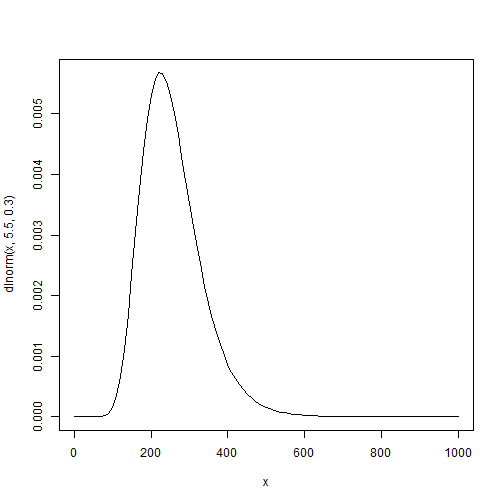
\includegraphics{Class6-figure/unnamed-chunk-19.png}
\caption{plot of chunk unnamed-chunk-19}
\end{figure}

\section{Example data}\label{example-data}

\begin{itemize}
\itemsep1pt\parskip0pt\parsep0pt
\item
  Example experiment: how long do people look at swear words
  vs.~non-swear words?

  \begin{itemize}
  \itemsep1pt\parskip0pt\parsep0pt
  \item
    Let's assume that the true means are 250 ms for non swear words and
    300 ms for swear words
  \end{itemize}
\item
  Let's generate data based on this assumption
\end{itemize}

\begin{Shaded}
\begin{Highlighting}[]
\KeywordTok{set.seed}\NormalTok{(}\StringTok{"11233"}\NormalTok{)}
\CommentTok{# 60 subjects}
\NormalTok{word_condition <-}\StringTok{ }\KeywordTok{factor}\NormalTok{(}\KeywordTok{c}\NormalTok{(}\KeywordTok{rep}\NormalTok{(}\StringTok{"swear word"}\NormalTok{, }\DecValTok{30}\NormalTok{), }\KeywordTok{rep}\NormalTok{(}\StringTok{"non swear word"}\NormalTok{, }\DecValTok{30}\NormalTok{)))}
\CommentTok{# rlnorm: Generate random samples from the lognormal distribution}
\NormalTok{fixation_time <-}\StringTok{ }\KeywordTok{c}\NormalTok{(}\KeywordTok{rlnorm}\NormalTok{(}\DataTypeTok{n =} \DecValTok{30}\NormalTok{, }\DataTypeTok{mean =} \KeywordTok{log}\NormalTok{(}\DecValTok{250}\NormalTok{), }\DataTypeTok{sd =} \NormalTok{.}\DecValTok{3}\NormalTok{), }\KeywordTok{rlnorm}\NormalTok{(}\DataTypeTok{n =} \DecValTok{30}\NormalTok{, }\DataTypeTok{mean =} \KeywordTok{log}\NormalTok{(}\DecValTok{265}\NormalTok{), }\DataTypeTok{sd =} \NormalTok{.}\DecValTok{3}\NormalTok{))}
\NormalTok{swear_exp <-}\StringTok{ }\KeywordTok{data.frame}\NormalTok{(word_condition, fixation_time)}
\end{Highlighting}
\end{Shaded}

\section{Running a linear model}\label{running-a-linear-model}

\begin{Shaded}
\begin{Highlighting}[]
\NormalTok{linear_model <-}\StringTok{ }\KeywordTok{lm}\NormalTok{(}\DataTypeTok{data =} \NormalTok{swear_exp, fixation_time ~}\StringTok{ }\NormalTok{word_condition)}
\KeywordTok{summary}\NormalTok{(linear_model)}
\end{Highlighting}
\end{Shaded}

\begin{verbatim}

Call:
lm(formula = fixation_time ~ word_condition, data = swear_exp)

Residuals:
   Min     1Q Median     3Q    Max 
-125.3  -62.9  -14.4   47.4  242.7 

Coefficients:
                         Estimate Std. Error t value Pr(>|t|)    
(Intercept)                 304.2       14.9   20.47   <2e-16 ***
word_conditionswear word    -50.8       21.0   -2.42    0.019 *  
---
Signif. codes:  0 '***' 0.001 '**' 0.01 '*' 0.05 '.' 0.1 ' ' 1

Residual standard error: 81.4 on 58 degrees of freedom
Multiple R-squared:  0.0917,    Adjusted R-squared:  0.076 
F-statistic: 5.85 on 1 and 58 DF,  p-value: 0.0187
\end{verbatim}

\section{Assumption test}\label{assumption-test}

\begin{Shaded}
\begin{Highlighting}[]
\KeywordTok{shapiro.test}\NormalTok{(}\KeywordTok{resid}\NormalTok{(linear_model))}
\end{Highlighting}
\end{Shaded}

\begin{verbatim}

    Shapiro-Wilk normality test

data:  resid(linear_model)
W = 0.9491, p-value = 0.01417
\end{verbatim}

\begin{itemize}
\itemsep1pt\parskip0pt\parsep0pt
\item
  Clearly not normal!
\item
  But notice how robust the analysis is. We still find the effect!
\item
  Nevertheless, better to run a proper model with log transformed values
  as the dependent vairable
\end{itemize}

\section{Running a log model}\label{running-a-log-model}

\begin{Shaded}
\begin{Highlighting}[]
\NormalTok{log_model <-}\StringTok{ }\KeywordTok{lm}\NormalTok{(}\DataTypeTok{data =} \NormalTok{swear_exp, }\KeywordTok{log}\NormalTok{(fixation_time) ~}\StringTok{ }\NormalTok{word_condition)}
\KeywordTok{summary}\NormalTok{(log_model)}
\end{Highlighting}
\end{Shaded}

\begin{verbatim}

Call:
lm(formula = log(fixation_time) ~ word_condition, data = swear_exp)

Residuals:
    Min      1Q  Median      3Q     Max 
-0.5636 -0.2392 -0.0132  0.1797  0.6319 

Coefficients:
                         Estimate Std. Error t value Pr(>|t|)    
(Intercept)                5.6835     0.0524  108.37   <2e-16 ***
word_conditionswear word  -0.1951     0.0742   -2.63    0.011 *  
---
Signif. codes:  0 '***' 0.001 '**' 0.01 '*' 0.05 '.' 0.1 ' ' 1

Residual standard error: 0.287 on 58 degrees of freedom
Multiple R-squared:  0.107, Adjusted R-squared:  0.0912 
F-statistic: 6.92 on 1 and 58 DF,  p-value: 0.0109
\end{verbatim}

\section{Assumption test}\label{assumption-test-1}

\begin{Shaded}
\begin{Highlighting}[]
\KeywordTok{shapiro.test}\NormalTok{(}\KeywordTok{resid}\NormalTok{(log_model))}
\end{Highlighting}
\end{Shaded}

\begin{verbatim}

    Shapiro-Wilk normality test

data:  resid(log_model)
W = 0.9823, p-value = 0.5325
\end{verbatim}

\section{How to interpret a log
model}\label{how-to-interpret-a-log-model}

\begin{itemize}
\itemsep1pt\parskip0pt\parsep0pt
\item
  Formula:
  $ln(y_{i}) = \beta_0 + \beta_1 x_{i1} + \beta_2 x_{i2} + \epsilon_i$
\item
  Let's rewrite that:
  $y_{i} = e^{\beta_0 + \beta_1 x_{i1} + \beta_2 x_{i2} + \epsilon_i} = e^{\beta_0} \times e^{\beta_1x_{i1}} \times e^{\beta_2x_{i2}}$

  \begin{itemize}
  \itemsep1pt\parskip0pt\parsep0pt
  \item
    If this confuses you: we are using the natural logarithm ($ln$; R
    somewhat confusingly calls it \texttt{log}) here. This is a
    logarithm to the base $e ~ 2.718$. Maybe you'll remember that
    $e^{ln(x)} = x$
  \end{itemize}
\item
  Log models are \emph{multiplicative} rather than \emph{additive}
\end{itemize}

\section{How to interpret a log model
(2)}\label{how-to-interpret-a-log-model-2}

\begin{itemize}
\itemsep1pt\parskip0pt\parsep0pt
\item
  Example: Our swear word fixation time study

  \begin{itemize}
  \itemsep1pt\parskip0pt\parsep0pt
  \item
    Fitted model: $ln(y_{i}) = 5.683 - .195 \times x_i$
  \item
    Remember: We're using treatment contrasts. $x_i$ is 0 for non swear
    words and 1 for swear words
  \item
    Predicted value for non swear words:
    $e^{5.683} \times e^{-.195 \times 0} = e^{5.683} =  293.82$
  \item
    Predicted value for swear words:
    $e^{5.683} \times e^{-.195 \times 1} = 293.82 \times e^{-.195} = 293.82 * .823 = 241.81$
  \end{itemize}
\item
  Conclusion: Fixation times on swear words were 17.7\% lower than
  fixation times on non swear words (\emph{b} = -.195, \emph{SE} = .074,
  \emph{t} = -2.63, \emph{p} = .011).
\end{itemize}

\section{Logistic regression}\label{logistic-regression}

\begin{itemize}
\itemsep1pt\parskip0pt\parsep0pt
\item
  What if we have a dichotomous dependent variable?

  \begin{itemize}
  \itemsep1pt\parskip0pt\parsep0pt
  \item
    Yes vs.~no, error vs.~no error, alive vs.~dead, pregnant vs.~not
    pregnant
  \end{itemize}
\item
  Our example (from A. Johnson): Factors that make (or don't make) you
  fail your driving test
\item
  90 candidates
\item
  Dependent variable: \texttt{Driving.Test}
\item
  Predictor variables:

  \begin{itemize}
  \itemsep1pt\parskip0pt\parsep0pt
  \item
    \texttt{Practice}: in hours
  \item
    \texttt{Emergency.Stop}: Whether the candidate performed the
    emergency stop (yes or no)
  \item
    \texttt{Examiner}: How difficult the examiner is (on a scale from 0
    = easy to 100 = extremely difficult)
  \item
    \texttt{Cold.Remedy}: How many doses of cold remedy the candidate
    had before the test
  \end{itemize}
\end{itemize}

\section{Where to start?}\label{where-to-start}

\begin{itemize}
\itemsep1pt\parskip0pt\parsep0pt
\item
  We would like to use our standard regression model
  $y_{i} = \beta_0 + \beta_1 x_{i1} + \beta_2 x_{i2} + \epsilon_i$
\item
  But our data are definitely not normally distributed (they aren't even
  continuous)
\item
  First step: represent the data as probabilities rather than Yes or No

  \begin{itemize}
  \itemsep1pt\parskip0pt\parsep0pt
  \item
    What's the probability of passing the test given that I've had (at
    most) 20 hours of practice, did my emergency stop, had at most an
    average examiner (50) and had only one cup of cold remedy?
  \item
    Probabilities are still weird: They only go from 0 to 1, and they
    also aren't great for linear relationships
  \item
    Let's try something else: odds
  \end{itemize}
\end{itemize}

\section{Probability and odds}\label{probability-and-odds}

\begin{itemize}
\itemsep1pt\parskip0pt\parsep0pt
\item
  Very popular in betting, since they make it easy to estimate the
  payout
\item
  $Odds = \frac{P}{1-P}$
\item
  For example:

  \begin{itemize}
  \itemsep1pt\parskip0pt\parsep0pt
  \item
    $P = .5$ gives you even odds $\frac{.5}{.5} = 1/1$
  \item
    $P = .25$ gives you $\frac{.25}{.75} = 1/3$
  \item
    $P = .75$ gives you $\frac{.75}{.25} = 3/1$
  \end{itemize}
\item
  Odds are nice because they aren't bounded, but for high probabilities
  they get very large very quickly
  ($P = .99 \Leftrightarrow Odds = 99/1$) and for small probabilities,
  they get very small very quickly
  ($P = .01 \Leftrightarrow Odds = 1/99$)
\item
  What to do?
\end{itemize}

\section{Log odds (logits)}\label{log-odds-logits}

\begin{itemize}
\itemsep1pt\parskip0pt\parsep0pt
\item
  Just transform our odds (just like we did with our continuous fixation
  time variable earlier) by taking the natural logarithm:
  $logit = ln(Odds) = ln(\frac{P}{1-P})$
\item
  Now we have a dependent measure that is suitable for linear
  relationships
\item
  Our new logistic regression model is
  $ln(\frac{P}{1-P}) = \beta_0 + \beta_1 x_{i1} + \beta_2 x_{i2} + \epsilon_i$
\item
  If we want to get back to probabilities, we can exponentiate both
  sides of the equation:
  $\frac{P}{1-P} = e^{\beta_0 + \beta_1 x_{i1} + \beta_2 x_{i2} + \epsilon_i}$
\item
  Solving this for $P$:
  $P = \frac{e^{\beta_0 + \beta_1 x_{i1} + \beta_2 x_{i2} + \epsilon_i}}{1 + e^{\beta_0 + \beta_1 x_{i1} + \beta_2 x_{i2} + \epsilon_i}} = \frac{1}{1 + e^{-(\beta_0 + \beta_1 x_{i1} + \beta_2 x_{i2} + \epsilon_i)}}$
\end{itemize}

\section{How do you fit a logistic regression
line?}\label{how-do-you-fit-a-logistic-regression-line}

\begin{itemize}
\itemsep1pt\parskip0pt\parsep0pt
\item
  Least squares won't work
\item
  We can evaluate the \textbf{likelihood} of the parameters instead
\item
  Probability: observations given parameters
\item
  Likelihood: parameters given observations
\end{itemize}

\section{Calculating likelihood}\label{calculating-likelihood}

\begin{itemize}
\itemsep1pt\parskip0pt\parsep0pt
\item
  Very simple example: Let's assume we have the following data from
  flipping a coin: $Y = (H H H T H T H H)$
\item
  Likelihood is the product of all the probabilities given a certain
  parameter value. In this case, we are trying different parameter
  values for the probability:

  \begin{itemize}
  \itemsep1pt\parskip0pt\parsep0pt
  \item
    We usually call the observed probability $p$, but since we are
    trying different population parameters, we'll give it a greek letter
    and call our population probability of observing ``heads'' (ignoring
    order) $\pi$ (that is, pi)
  \end{itemize}
\item
  $\pi = .5$:
  $L(Y|\pi = .5) = .5 \times .5 \times .5 \times .5 \times .5 \times .5 \times .5 \times .5 = .5^8 = .00039$
\item
  $\pi = .25$:
  $L(Y|\pi = .35) = .25 \times .25 \times .25 \times .75 \times .25 \times .75 \times .25 \times .25 = .25^6 \times .75^2 = .00014$

  \begin{itemize}
  \itemsep1pt\parskip0pt\parsep0pt
  \item
    $\pi = .25$ has a lower likelihood than $\pi = .5$.
  \end{itemize}
\item
  Let's try $\pi = .75$:
  $L(Y|\pi = .75) = .75 \times .75 \times .75 \times .25 \times .75 \times .25 \times .75 \times .75 = .75^6 \times .25^2 = .00111$

  \begin{itemize}
  \itemsep1pt\parskip0pt\parsep0pt
  \item
    This is the highest one yet.
  \end{itemize}
\end{itemize}

\section{The likelihood function for logistic
regression}\label{the-likelihood-function-for-logistic-regression}

\begin{itemize}
\itemsep1pt\parskip0pt\parsep0pt
\item
  Do you see a pattern here? For each element $Y_i$ in $Y$, the
  likelihood of $\pi$ is either

  \begin{itemize}
  \itemsep1pt\parskip0pt\parsep0pt
  \item
    $L(Y_i|\pi) = \pi$ if $Y_i = H$, (e.g. $.75$ for $\pi = .75$), or
  \item
    $L(Y_i|\pi) = 1 - \pi$ if $Y_i = T$, (e.g. $.25$ for $\pi = .75$)
  \end{itemize}
\item
  Then you get the likelihood for the full data set $Y$ by multiplying
  all the individual likelihoods

  \begin{itemize}
  \itemsep1pt\parskip0pt\parsep0pt
  \item
    $L(Y|\pi) = \prod_{i = 1}^N{L(Y_i|\pi)}$
  \end{itemize}
\item
  You can simplify this a bit if you replace H with 1 and T with 0:

  \begin{itemize}
  \itemsep1pt\parskip0pt\parsep0pt
  \item
    $L(Y_i|\pi) = \pi^{Y_i} \times (1-\pi)^{(1-Y_i)}$
  \item
    And combining the two equations above:

    \begin{itemize}
    \itemsep1pt\parskip0pt\parsep0pt
    \item
      $L(Y|\pi) = \prod_{i = 1}^N\pi^{Y_i} \times (1-\pi)^{(1-Y_i)}$
    \end{itemize}
  \end{itemize}
\end{itemize}

\section{Maximum likelihood}\label{maximum-likelihood}

\begin{itemize}
\itemsep1pt\parskip0pt\parsep0pt
\item
  Likelihood gets a little unwieldy -- lots of very small numbers

  \begin{itemize}
  \itemsep1pt\parskip0pt\parsep0pt
  \item
    Solution: take the log (who would have thought?)

    \begin{itemize}
    \itemsep1pt\parskip0pt\parsep0pt
    \item
      Added bonus: Now our multiplication becomes a sum (remember that
      from calculus?)
      $log\;likelihood = \sum_{i = 1}^N Y_i\times ln(\pi) + (1-Y_i)\times ln(1-\pi)$
    \end{itemize}
  \end{itemize}
\item
  Now we can simply try different values of $\pi$ until we find the one
  with the maximum likelihood

  \begin{itemize}
  \itemsep1pt\parskip0pt\parsep0pt
  \item
    Remember that in logistic regression, $\pi$ is defined by our
    regression equation:
    $\pi = \frac{1}{1 + e^{-(\beta_0 + \beta_1 x_{i1} + \beta_2 x_{i2} + \epsilon_i)}}$
  \item
    Instead of simply trying different values of $\pi$, we have to try
    different values for $\beta_0$, $\beta_1$, etc. and compute $\pi$.
    This gets to be quite a lot of work.
  \item
    Trying different values might not seem particularly elegant, but
    this is essentially what R or SPSS do -- no simple solution like
    with least-squares regression or ANOVA exists
  \item
    This is (relatively) processing-intensive. One reason why
    psychologists didn't use logistic regression in the
    statistics-by-hand era.
  \end{itemize}
\end{itemize}

\section{Log likelihood as an indicator of model
fit}\label{log-likelihood-as-an-indicator-of-model-fit}

\begin{itemize}
\itemsep1pt\parskip0pt\parsep0pt
\item
  The log likelihood (LL) of the final model is an indicator of how well
  the model fit the data, just like $R^2$.

  \begin{itemize}
  \itemsep1pt\parskip0pt\parsep0pt
  \item
    In fact, there are several ways to estimate $R^2$ from the log
    likelihood
  \end{itemize}
\item
  Log likelihood also enables us to make model comparisons

  \begin{itemize}
  \itemsep1pt\parskip0pt\parsep0pt
  \item
    The test statistic in that case is $\chi^2$ -- more about that later
  \end{itemize}
\item
  Another measure is \emph{deviance}, which is simply $-2$*LL

  \begin{itemize}
  \itemsep1pt\parskip0pt\parsep0pt
  \item
    Conceptually, deviance is like the residual variance.

    \begin{itemize}
    \itemsep1pt\parskip0pt\parsep0pt
    \item
      In the case of deviance, lower is better, of course.
    \end{itemize}
  \end{itemize}
\item
  Closely related to this is Akaike's Information Criterion (AIC), which
  is -2LL+2*number of parameters (lower is better, so adding parameters
  makes the AIC worse)
\end{itemize}

\section{Enough maths, let's just run this
model}\label{enough-maths-lets-just-run-this-model}

\begin{itemize}
\itemsep1pt\parskip0pt\parsep0pt
\item
  These are our data (first 6 rows):
\end{itemize}

\begin{Shaded}
\begin{Highlighting}[]
\NormalTok{driving_tests <-}\StringTok{ }\KeywordTok{read.csv}\NormalTok{(}\StringTok{"driving_tests.csv"}\NormalTok{)}
\KeywordTok{kable}\NormalTok{(}\KeywordTok{head}\NormalTok{(driving_tests))}
\end{Highlighting}
\end{Shaded}

\begin{longtable}[c]{@{}lrrrr@{}}
\toprule\addlinespace
Driving.Test & Practice & Emergency.Stop & Examiner & Cold.Remedy
\\\addlinespace
\midrule\endhead
Yes & 45 & 1 & 23 & 0
\\\addlinespace
No & 18 & 0 & 88 & 0
\\\addlinespace
Yes & 25 & 0 & 15 & 0
\\\addlinespace
Yes & 30 & 1 & 4 & 0
\\\addlinespace
No & 20 & 1 & 82 & 5
\\\addlinespace
No & 25 & 0 & 75 & 0
\\\addlinespace
\bottomrule
\end{longtable}

\section{Fitting the model}\label{fitting-the-model}

\begin{itemize}
\itemsep1pt\parskip0pt\parsep0pt
\item
  We use \texttt{glm} instead of \texttt{lm} (short for generalised
  linear model)
\item
  We tell \texttt{glm} that our data are binomial and we want to use the
  logit function as the link
\item
  Note that, for simplicity, we're not investigating interactions here
  (let's assume that in this example we simply aren't interested in
  them)
\end{itemize}

\begin{Shaded}
\begin{Highlighting}[]
\NormalTok{driving_glm <-}\StringTok{ }\KeywordTok{glm}\NormalTok{(}\DataTypeTok{data =} \NormalTok{driving_tests, }\DataTypeTok{formula =} \NormalTok{Driving.Test ~}\StringTok{ }\NormalTok{Practice +}\StringTok{ }\NormalTok{Emergency.Stop +}\StringTok{ }\NormalTok{Examiner +}\StringTok{ }\NormalTok{Cold.Remedy, }\DataTypeTok{family =} \KeywordTok{binomial}\NormalTok{(}\DataTypeTok{link =} \StringTok{"logit"}\NormalTok{))}
\end{Highlighting}
\end{Shaded}

\section{Model summary}\label{model-summary}

\begin{Shaded}
\begin{Highlighting}[]
\KeywordTok{summary}\NormalTok{(driving_glm)}
\end{Highlighting}
\end{Shaded}

\begin{verbatim}

Call:
glm(formula = Driving.Test ~ Practice + Emergency.Stop + Examiner + 
    Cold.Remedy, family = binomial(link = "logit"), data = driving_tests)

Deviance Residuals: 
   Min      1Q  Median      3Q     Max  
-2.266  -0.732  -0.301   0.663   2.021  

Coefficients:
               Estimate Std. Error z value Pr(>|z|)    
(Intercept)     -2.4057     1.1867   -2.03   0.0426 *  
Practice         0.1296     0.0303    4.28  1.9e-05 ***
Emergency.Stop   0.0494     0.5912    0.08   0.9334    
Examiner        -0.0348     0.0130   -2.68   0.0074 ** 
Cold.Remedy     -0.0765     0.1685   -0.45   0.6501    
---
Signif. codes:  0 '***' 0.001 '**' 0.01 '*' 0.05 '.' 0.1 ' ' 1

(Dispersion parameter for binomial family taken to be 1)

    Null deviance: 124.366  on 89  degrees of freedom
Residual deviance:  82.572  on 85  degrees of freedom
AIC: 92.57

Number of Fisher Scoring iterations: 5
\end{verbatim}

\section{Model summary explained}\label{model-summary-explained}

\begin{itemize}
\itemsep1pt\parskip0pt\parsep0pt
\item
  Deviance residuals:

  \begin{itemize}
  \itemsep1pt\parskip0pt\parsep0pt
  \item
    For these, we calculate the deviance separately for each case and
    then take the square root. We also change the sign depending on
    whether the observed case was 1 or 0:
  \item
    $d_i = s_i \sqrt{-2(Y_i\times ln(\pi) + (1-Y_i)\times ln(1-\pi))}$

    \begin{itemize}
    \itemsep1pt\parskip0pt\parsep0pt
    \item
      with $s_i = 1$ if $Y_i = 1$ and $s_i = -1$ if $Y_i = 0$
    \end{itemize}
  \end{itemize}
\end{itemize}

\section{How to interpret logistic regression
residuals}\label{how-to-interpret-logistic-regression-residuals}

\begin{itemize}
\itemsep1pt\parskip0pt\parsep0pt
\item
  Can't test if they are normally distributed (because they are not)
\item
  But look out for very large residuals
\item
  You can get standardised residuals using \texttt{rstandard}.

  \begin{itemize}
  \itemsep1pt\parskip0pt\parsep0pt
  \item
    Look out for cases that are far away from 0.
  \end{itemize}
\end{itemize}

\begin{Shaded}
\begin{Highlighting}[]
\NormalTok{driving_residuals <-}\StringTok{ }\KeywordTok{rstandard}\NormalTok{(driving_glm)}
\KeywordTok{plot}\NormalTok{(driving_residuals)}
\end{Highlighting}
\end{Shaded}

\begin{figure}[htbp]
\centering
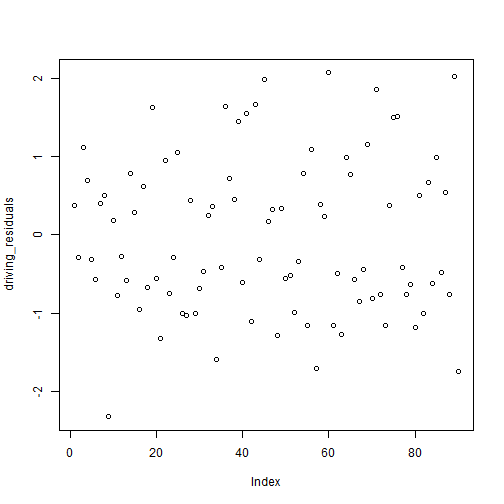
\includegraphics{Class6-figure/unnamed-chunk-28.png}
\caption{plot of chunk unnamed-chunk-28}
\end{figure}

\section{Model summary explained (2)}\label{model-summary-explained-2}

\begin{itemize}
\itemsep1pt\parskip0pt\parsep0pt
\item
  The coefficients
\end{itemize}

\textbar{} \textbar{} Estimate\textbar{} Std. Error\textbar{} z
value\textbar{} Pr(\textgreater{}\textbar{}z\textbar{})\textbar{}
\textbar{}:--------------\textbar{}--------:\textbar{}----------:\textbar{}-------:\textbar{}------------------:\textbar{}
\textbar{}(Intercept) \textbar{} -2.4057\textbar{} 1.1867\textbar{}
-2.0272\textbar{} 0.0426\textbar{} \textbar{}Practice \textbar{}
0.1296\textbar{} 0.0303\textbar{} 4.2796\textbar{} 0.0000\textbar{}
\textbar{}Emergency.Stop \textbar{} 0.0494\textbar{} 0.5912\textbar{}
0.0836\textbar{} 0.9334\textbar{} \textbar{}Examiner \textbar{}
-0.0348\textbar{} 0.0130\textbar{} -2.6794\textbar{} 0.0074\textbar{}
\textbar{}Cold.Remedy \textbar{} -0.0765\textbar{} 0.1685\textbar{}
-0.4537\textbar{} 0.6501\textbar{} - Analogous to linear regression:
\emph{b} value, \emph{SE}, significance test - Using the \textbf{Wald}
statistic instead of \emph{t} tests - $z = \frac{b}{SE_b}$ - Can be
interpreted like \emph{z} values from a standard normal distribution
(that's how the \emph{p}-value is computed)

\section{Interpreting the b values}\label{interpreting-the-b-values}

\begin{itemize}
\itemsep1pt\parskip0pt\parsep0pt
\item
  If you take the exponential of the coefficients (using \texttt{exp()}
  or \texttt{e\^{}} in R), you get an \textbf{odds ratio}
\item
  Odds ratio = Odds after a unit change in the predictor divided by the
  original odds
\item
  Example: According to our model, each hour of practice increases the
  odds of passing the test by a factor of $e^{0.12959} = 1.1384$

  \begin{itemize}
  \itemsep1pt\parskip0pt\parsep0pt
  \item
    e.g.~if the odds were even (1/1) for X hours of practice, they would
    be slightly better than even (1.138/1) for X+1 hours of practice
  \end{itemize}
\item
  On the other hand, each ``unit'' of examiner difficulty decreases the
  odds of passing the test by a factor of $e^{-0.03485} = 0.9658$

  \begin{itemize}
  \itemsep1pt\parskip0pt\parsep0pt
  \item
    e.g.~if the odds were even (1/1) for an instructor with a difficulty
    of X, they would be slightly worse than even (0.9658/1) for an
    instructor with a difficulty of X+1
  \end{itemize}
\end{itemize}

\section{Model summary explained (2)}\label{model-summary-explained-2-1}

\begin{itemize}
\itemsep1pt\parskip0pt\parsep0pt
\item
  Null deviance: deviance from a model that estimates all values using
  the overall probability of passing the test (without taking into
  account the 4 predictors)
\item
  Residual deviance: deviance from the current model (note that we're
  losing 4 df due to the 4 predictors)
\item
  AIC: residual deviance + 2*model df (note that the model has 5 df,
  including one for the intercept)
\end{itemize}

\section{Model comparisons (LRT)}\label{model-comparisons-lrt}

\begin{itemize}
\itemsep1pt\parskip0pt\parsep0pt
\item
  Deviance has some neat properties

  \begin{itemize}
  \itemsep1pt\parskip0pt\parsep0pt
  \item
    We can compare likelihoods just like we compared mean squares in the
    F-test: by dividing them
  \item
    That is, we compute a likelihood ratio:
    $LR = \frac{L_{baseline}}{L_{new}}$, where \emph{baseline} is the
    simpler model and \emph{new} the more complex model.
  \item
    Now we can convert this likelihood ratio into a deviance:
    $deviance_{LR} = -2\frac{ln(L_{baseline})}{ln(L_{new})} = deviance_{baseline} - deviance_{new}$
  \item
    And now the most fun part: If the $H_0$ that the two models explain
    the data equally well is true, this likelihood-ratio deviance is
    distributed according to a $\chi^2$ distribution.
  \item
    The $\chi^2$ distribution has one parameter, degrees of freedom
  \item
    $df = k_{new}$ - $k_{baseline}$, where $k$ is the number of
    parameters (including the intercept)
  \end{itemize}
\end{itemize}

\section{Model comparisons}\label{model-comparisons}

\begin{itemize}
\itemsep1pt\parskip0pt\parsep0pt
\item
  Now we can get a \emph{p}-value! This is called the \textbf{Likelihood
  ratio test (LRT)}
\item
  So, if we want to test if the model is better than a model with just
  the intercept, we can do an LRT
\item
  $\chi^2 = deviance_{null} - deviance_{model} = 124.366 - 82.572 = 41.794$
\item
  $df = k_{null} - k_{model} = 89 - 85 = 4$
\item
  $p(\chi^2(4) \geq 41.794) < .01$
\item
  This is equivalent to the overall F-test for the model.
\end{itemize}

\section{Model comparisons (2)}\label{model-comparisons-2}

\begin{itemize}
\itemsep1pt\parskip0pt\parsep0pt
\item
  We can use model comparisons to test how specific predictors
  contribute to the whole model (analogous to the F-tests in linear
  regression)
\item
  For this, you can use the \texttt{Anova} command from the \texttt{car}
  package:
\end{itemize}

\begin{Shaded}
\begin{Highlighting}[]
\KeywordTok{library}\NormalTok{(car)}
\KeywordTok{Anova}\NormalTok{(driving_glm)}
\end{Highlighting}
\end{Shaded}

\begin{verbatim}
Analysis of Deviance Table (Type II tests)

Response: Driving.Test
               LR Chisq Df Pr(>Chisq)    
Practice          28.93  1    7.5e-08 ***
Emergency.Stop     0.01  1     0.9334    
Examiner           8.11  1     0.0044 ** 
Cold.Remedy        0.22  1     0.6421    
---
Signif. codes:  0 '***' 0.001 '**' 0.01 '*' 0.05 '.' 0.1 ' ' 1
\end{verbatim}

\section{Model comparisons (3)}\label{model-comparisons-3}

\begin{itemize}
\itemsep1pt\parskip0pt\parsep0pt
\item
  This analysis of deviance follows the same logic as the ANOVA in the
  linear regression case
\item
  You can do Type I, Type II, and Type III LRT tests (they are not sums
  of squares in this case)
\item
  The LRTs are better tests than the Wald tests, since the Wald tests
  might be prone to overinflating the SE, leading to Type II error.
\item
  You can also use the LRT to directly compare a model to another (just
  like in the linear regression case). For this, you can use the
  \texttt{anova} command (lower case \texttt{a}).
\end{itemize}

\section{Diagnostics and assumption
tests}\label{diagnostics-and-assumption-tests}

\begin{itemize}
\itemsep1pt\parskip0pt\parsep0pt
\item
  We do not assume normality (so nothing to test for that one)
\item
  All the influence measures from linear regression work in logistic
  regression as well

  \begin{itemize}
  \itemsep1pt\parskip0pt\parsep0pt
  \item
    See Class 5 notes for explanations and criteria
  \end{itemize}
\end{itemize}

\begin{Shaded}
\begin{Highlighting}[]
\KeywordTok{kable}\NormalTok{(}\KeywordTok{head}\NormalTok{(}\KeywordTok{influence.measures}\NormalTok{(driving_glm)$infmat))}
\end{Highlighting}
\end{Shaded}

\begin{longtable}[c]{@{}rrrrrrrrr@{}}
\toprule\addlinespace
dfb.1\_ & dfb.Prct & dfb.Em.S & dfb.Exmn & dfb.Cl.R & dffit & cov.r &
cook.d & hat
\\\addlinespace
\midrule\endhead
-0.0181 & 0.0485 & 0.0157 & -0.0336 & -0.0035 & 0.0640 & 1.0830 & 0.0004
& 0.0284
\\\addlinespace
-0.0180 & 0.0302 & 0.0189 & -0.0312 & 0.0161 & -0.0494 & 1.0845 & 0.0002
& 0.0268
\\\addlinespace
0.3418 & -0.0665 & -0.2944 & -0.2826 & 0.0037 & 0.4241 & 1.1197 & 0.0232
& 0.1221
\\\addlinespace
0.0672 & 0.0324 & 0.0238 & -0.1501 & 0.0108 & 0.1822 & 1.1013 & 0.0036 &
0.0640
\\\addlinespace
-0.0032 & 0.0268 & -0.0175 & -0.0211 & -0.0407 & -0.0615 & 1.0935 &
0.0004 & 0.0357
\\\addlinespace
-0.0468 & 0.0535 & 0.0690 & -0.0643 & 0.0457 & -0.1271 & 1.0905 & 0.0017
& 0.0462
\\\addlinespace
\bottomrule
\end{longtable}

\section{Diagnostics and assumption tests
(2)}\label{diagnostics-and-assumption-tests-2}

\begin{itemize}
\itemsep1pt\parskip0pt\parsep0pt
\item
  Multicollinearity:
\item
  You can get Variance Inflation Factors (VIFs)

  \begin{itemize}
  \itemsep1pt\parskip0pt\parsep0pt
  \item
    Again, see Class 5 notes for explanations and criteria
  \end{itemize}
\end{itemize}

\begin{Shaded}
\begin{Highlighting}[]
\KeywordTok{vif}\NormalTok{(driving_glm)}
\end{Highlighting}
\end{Shaded}

\begin{verbatim}
      Practice Emergency.Stop       Examiner    Cold.Remedy 
         1.057          1.062          1.199          1.100 
\end{verbatim}

\section{Linearity}\label{linearity}

\begin{itemize}
\itemsep1pt\parskip0pt\parsep0pt
\item
  This is a new one: Test if the effects of the predictors on the logits
  are actually linear
\item
  How to do it: run a model that includes interactions between each
  \emph{continuous} predictor and its logarithm
\item
  Test each interaction in a separate model
\item
  If you have 0s in your data, you might need to replace them by a very
  small value since log(0) = -Inf
\item
  If the interaction is significant, linearity is violated
\end{itemize}

\section{Linearity (2)}\label{linearity-2}

\begin{Shaded}
\begin{Highlighting}[]
\CommentTok{# remove 0s by adding a very small number to Cold.Remedy}
\CommentTok{# test each factor in a separate model}
\NormalTok{driving_tests$Cold.Remedy_no_0 <-}\StringTok{ }\NormalTok{driving_tests$Cold.Remedy +}\StringTok{ }\DecValTok{1}
\NormalTok{driving_glm_linearity <-}\StringTok{ }\KeywordTok{glm}\NormalTok{(}\DataTypeTok{data =} \NormalTok{driving_tests, }\DataTypeTok{formula =} \NormalTok{Driving.Test ~}\StringTok{ }\NormalTok{Practice +}\StringTok{ }\NormalTok{Emergency.Stop +}\StringTok{ }\NormalTok{Examiner +}\StringTok{ }\NormalTok{Cold.Remedy_no_0 +}\StringTok{ }\NormalTok{Practice:}\KeywordTok{log}\NormalTok{(Practice) +}\StringTok{ }\NormalTok{Examiner:}\KeywordTok{log}\NormalTok{(Examiner) +}\StringTok{ }\NormalTok{Cold.Remedy_no_0:}\KeywordTok{log}\NormalTok{(Cold.Remedy_no_0), }\DataTypeTok{family =} \KeywordTok{binomial}\NormalTok{(}\DataTypeTok{link =} \StringTok{"logit"}\NormalTok{))}
\end{Highlighting}
\end{Shaded}

\section{Linearity(3)}\label{linearity3}

\begin{Shaded}
\begin{Highlighting}[]
\KeywordTok{kable}\NormalTok{(}\KeywordTok{coef}\NormalTok{(}\KeywordTok{summary}\NormalTok{(driving_glm_linearity)))}
\end{Highlighting}
\end{Shaded}

\textbar{} \textbar{} Estimate\textbar{} Std. Error\textbar{} z
value\textbar{} Pr(\textgreater{}\textbar{}z\textbar{})\textbar{}
\textbar{}:--------------------------------------\textbar{}--------:\textbar{}----------:\textbar{}-------:\textbar{}------------------:\textbar{}
\textbar{}(Intercept) \textbar{} -11.1434\textbar{} 6.2465\textbar{}
-1.7840\textbar{} 0.0744\textbar{} \textbar{}Practice \textbar{}
0.9649\textbar{} 0.6933\textbar{} 1.3919\textbar{} 0.1640\textbar{}
\textbar{}Emergency.Stop \textbar{} -0.2542\textbar{} 0.6679\textbar{}
-0.3806\textbar{} 0.7035\textbar{} \textbar{}Examiner \textbar{}
-0.4805\textbar{} 0.2816\textbar{} -1.7062\textbar{} 0.0880\textbar{}
\textbar{}Cold.Remedy\_no\_0 \textbar{} 6.0141\textbar{}
2.4454\textbar{} 2.4593\textbar{} 0.0139\textbar{}
\textbar{}Practice:log(Practice) \textbar{} -0.1784\textbar{}
0.1523\textbar{} -1.1715\textbar{} 0.2414\textbar{}
\textbar{}Examiner:log(Examiner) \textbar{} 0.0902\textbar{}
0.0577\textbar{} 1.5642\textbar{} 0.1178\textbar{}
\textbar{}Cold.Remedy\_no\_0:log(Cold.Remedy\_no\_0) \textbar{}
-3.0393\textbar{} 1.2698\textbar{} -2.3935\textbar{} 0.0167\textbar{} -
There is an issue with the linearity of Cold.Remedy, suggesting that
this variable might have to be transformed/coded as a factor/etc. -
Maybe this is why we don't see a significant effect?

\section{Reporting it}\label{reporting-it}

A logistic regression was conducted where the dependent variable was
passing a driving test and the predictor variables were hours of
practice, whether an emergency stop was successfully executed, how much
the examiner was difficult, and amount of `cold remedy drinks' consumed.
90 cases were examined and the model was found to significantly predict
whether the test was passed (omnibus chi-square = 41.79, df=4,
p\textless{}.001). that practice and examiner were the only two
variables that reliably predicted if the driving test was passed.
Increases in practice was associated with increased rate of passing
(odds of passing increased by 1.14 per hour of practice, \emph{b} =
.130, SE = .03, \emph{z} = 4.28, \emph{p} \textless{} .01). Increases in
the examiner being an difficult reduced the rate of passing (odds of
passing decreased by 0.96 per unit of difficulty rating, \emph{b} =
-.00349, SE = .013, \emph{z} = -2.679, \emph{p} \textless{} .01). None
of the other predictors reached significance (all \emph{p}s
\textgreater{} .05). There were no issues due to multicollinearity or
influential cases, however, the linearity assumption was violated for
the cold remedy drinks predictor.

\section{Linear mixed models (LMMs)}\label{linear-mixed-models-lmms}

\begin{itemize}
\itemsep1pt\parskip0pt\parsep0pt
\item
  The final step to greatness!

  \begin{itemize}
  \itemsep1pt\parskip0pt\parsep0pt
  \item
    Note that we can really only scratch the surface here.
  \end{itemize}
\item
  Main issue:

  \begin{itemize}
  \itemsep1pt\parskip0pt\parsep0pt
  \item
    We know how to to regressions for continuous and discrete DVs now
  \item
    We know what the regression equivalent of a between-subjects ANOVA
    is and we can take the regression analysis much further than an
    ANOVA or ANCOVA would let us
  \item
    However:

    \begin{itemize}
    \itemsep1pt\parskip0pt\parsep0pt
    \item
      What if we have a within-subject or repeated measures design?
    \item
      What if there is some other underlying correlation in the data

      \begin{itemize}
      \itemsep1pt\parskip0pt\parsep0pt
      \item
        e.g.~data collected from students in different classes in
        different schools

        \begin{itemize}
        \itemsep1pt\parskip0pt\parsep0pt
        \item
          Surely the classes and schools share some variance -- how to
          account for that?
        \end{itemize}
      \end{itemize}
    \end{itemize}
  \end{itemize}
\end{itemize}

\section{Moving from linear regression to linear mixed
models}\label{moving-from-linear-regression-to-linear-mixed-models}

\begin{itemize}
\itemsep1pt\parskip0pt\parsep0pt
\item
  In repeated-measures ANOVA, we've dealt with within-subjects effects
  by removing the variance due to subject differences from the error

  \begin{itemize}
  \itemsep1pt\parskip0pt\parsep0pt
  \item
    Essentially, we have added a ``subject'' factor to the model
  \item
    Linear mixed models enable us to do the same thing for regression
    analyses
  \end{itemize}
\end{itemize}

\section{Problem: how to add subject as a
factor}\label{problem-how-to-add-subject-as-a-factor}

\begin{itemize}
\itemsep1pt\parskip0pt\parsep0pt
\item
  We could simply add a ``subject'' factor to the predictors

  \begin{itemize}
  \itemsep1pt\parskip0pt\parsep0pt
  \item
    This would reflect the systematic differences between subjects

    \begin{itemize}
    \itemsep1pt\parskip0pt\parsep0pt
    \item
      But that's not quite right: how do we deal with a factor with 40
      levels?

      \begin{itemize}
      \itemsep1pt\parskip0pt\parsep0pt
      \item
        Also, we want to generalise our model to more than those 40
        subjects that are in the analysis
      \item
        How do we do that?
      \end{itemize}
    \end{itemize}
  \item
    Subject is really like a random variable: we get a different set
    each time we run the experiment
  \item
    Instead of analysing the subject effect in a generalisable way, we
    really just want to get rid of the subject variance in the most
    efficient way possible
  \end{itemize}
\end{itemize}

\section{Problem: how to add subject as a factor
(2)}\label{problem-how-to-add-subject-as-a-factor-2}

\begin{itemize}
\itemsep1pt\parskip0pt\parsep0pt
\item
  Fixed effects vs.~random effects

  \begin{itemize}
  \itemsep1pt\parskip0pt\parsep0pt
  \item
    Fixed effects: repeatable, generalisable (e.g.~experiment condition)
  \item
    Random effects: non-repeatable, sampled from a general population
  \item
    Mixed effects models include both fixed and random effects
  \end{itemize}
\item
  Another issue with including subject as a fixed effect:

  \begin{itemize}
  \itemsep1pt\parskip0pt\parsep0pt
  \item
    Each subject would take up a degree of freedom
  \item
    That would majorly impact the power of our analysis
  \item
    LMMs solve this issue by a procedure called \textbf{shrinkage}
  \end{itemize}
\end{itemize}

\section{Shrinkage}\label{shrinkage}

\begin{itemize}
\itemsep1pt\parskip0pt\parsep0pt
\item
  Conceptually, LMMs allow subjects to have individual effects (e.g.~in
  an eye-tracking experiment subject 1 might have an intercept of 200
  ms, while subject 2 might have an intercept of 210 ms), but they pull
  each subject's effects towards an underlying distribution of subject
  effects
\item
  This reflects the idea that if 20 other subjects have intercepts
  between 180 and 220 ms, the current subject is unlikely to have an
  intercept of 400 ms, even though it looks like that from the data
\item
  Shrinkage also helps majorly with missing data issues (although it
  won't fix them for you!)
\item
  The downside of shrinkage is that it isn't clear what the
  df\_\{Error\} should be

  \begin{itemize}
  \itemsep1pt\parskip0pt\parsep0pt
  \item
    This leads to some issues later on.
  \end{itemize}
\end{itemize}

\section{Example}\label{example-4}

A PhD student wants to investigate whether our mood affects how we react
to visual scenes. In order to do this, she showed 40 subjects a total of
40 scenes. There are two version of each scene: one contains people, the
other one doesn't -- everything else is identical. The PhD student spent
a considerable amount of time taking photos to ensure this (until her
supervisor got a bit impatient). Before the experiment, all subjects
were asked to rate their current mood on a scale from 0 (very sad) to
100 (very happy). They then looked at each scene and rated how much they
liked it on a scale from 0 (hate it) to 20 (love it). The student's
hypothesis is that if you are happy, you should want to see scenes with
people. If you are unhappy, you should prefer scenes without people. The
data are given below. Will the student find what she is looking for? Or
will she have to start from scratch and be in even more trouble with her
supervisor?

\section{Example Data}\label{example-data-1}

\begin{itemize}
\itemsep1pt\parskip0pt\parsep0pt
\item
  Subject: Subject ID (1-40)
\item
  Item: Item ID (1-40)
\item
  Scene Type: within-item factor (``no people'' vs. ``people'')
\item
  Mood: between-subject factor (scale from 0--100)
\item
  Rating: Dependent variable (scale from 0 to 20)
\end{itemize}

\begin{Shaded}
\begin{Highlighting}[]
\CommentTok{# Start by loading the data}
\NormalTok{scene_liking <-}\StringTok{ }\KeywordTok{read.csv}\NormalTok{(}\StringTok{"Class 6 exercise data.csv"}\NormalTok{)}
\end{Highlighting}
\end{Shaded}

\section{Looking at the data}\label{looking-at-the-data}

\begin{Shaded}
\begin{Highlighting}[]
\KeywordTok{kable}\NormalTok{(}\KeywordTok{head}\NormalTok{(scene_liking))}
\end{Highlighting}
\end{Shaded}

\begin{longtable}[c]{@{}rrlrr@{}}
\toprule\addlinespace
subject & item & scene & mood & rating
\\\addlinespace
\midrule\endhead
1 & 1 & people & 55 & 12.2
\\\addlinespace
1 & 2 & no people & 55 & 8.5
\\\addlinespace
1 & 3 & people & 55 & 10.7
\\\addlinespace
1 & 4 & no people & 55 & 12.0
\\\addlinespace
1 & 5 & people & 55 & 12.3
\\\addlinespace
1 & 6 & no people & 55 & 16.0
\\\addlinespace
\bottomrule
\end{longtable}

\section{Looking at the data (2)}\label{looking-at-the-data-2}

\begin{Shaded}
\begin{Highlighting}[]
\KeywordTok{str}\NormalTok{(scene_liking)}
\end{Highlighting}
\end{Shaded}

\begin{verbatim}
'data.frame':   1600 obs. of  5 variables:
 $ subject: int  1 1 1 1 1 1 1 1 1 1 ...
 $ item   : int  1 2 3 4 5 6 7 8 9 10 ...
 $ scene  : Factor w/ 2 levels "no people","people": 2 1 2 1 2 1 2 1 2 1 ...
 $ mood   : int  55 55 55 55 55 55 55 55 55 55 ...
 $ rating : num  12.2 8.5 10.7 12 12.3 16 8.2 13.2 6.7 6.9 ...
\end{verbatim}

\begin{Shaded}
\begin{Highlighting}[]
\CommentTok{# We should set subject and item to be factors}
\NormalTok{scene_liking$subject <-}\StringTok{ }\KeywordTok{factor}\NormalTok{(scene_liking$subject)}
\NormalTok{scene_liking$item <-}\StringTok{ }\KeywordTok{factor}\NormalTok{(scene_liking$item)}
\end{Highlighting}
\end{Shaded}

\section{Calculating means}\label{calculating-means}

\begin{itemize}
\itemsep1pt\parskip0pt\parsep0pt
\item
  Let's get condition means for scene type
\item
  We can't really use \texttt{ez} for this, since we have two random
  variables
\item
  In theory, we could report means by subject or means by item
\item
  Either one would be fine, but usually people report subject means.

  \begin{itemize}
  \itemsep1pt\parskip0pt\parsep0pt
  \item
    We use \texttt{melt} and \texttt{cast} from the \texttt{reshape}
    package to calculate the means
  \end{itemize}
\end{itemize}

\begin{Shaded}
\begin{Highlighting}[]
\KeywordTok{library}\NormalTok{(reshape)}
\CommentTok{# set rating as the dependent (measure) variable}
\NormalTok{scene_liking.m <-}\StringTok{ }\KeywordTok{melt}\NormalTok{(scene_liking, }\DataTypeTok{measure =} \StringTok{"rating"}\NormalTok{)}
\CommentTok{# collapse over item; calculate means}
\NormalTok{scene_liking.c <-}\StringTok{ }\KeywordTok{cast}\NormalTok{(scene_liking.m, subject +}\StringTok{ }\NormalTok{mood +}\StringTok{ }\NormalTok{scene ~}\StringTok{ }\NormalTok{variable, mean)}
\end{Highlighting}
\end{Shaded}

\section{Calculating means (2)}\label{calculating-means-2}

\begin{Shaded}
\begin{Highlighting}[]
\KeywordTok{head}\NormalTok{(scene_liking.c)}
\end{Highlighting}
\end{Shaded}

\begin{verbatim}
  subject mood     scene rating
1       1   55 no people  10.87
2       1   55    people  10.36
3       2   56 no people  10.91
4       2   56    people  10.79
5       3   16 no people  12.33
6       3   16    people  11.54
\end{verbatim}

\section{Calculating means (2)}\label{calculating-means-2-1}

\begin{itemize}
\itemsep1pt\parskip0pt\parsep0pt
\item
  Now we can use this to calculate our means for the scene condition
\end{itemize}

\begin{Shaded}
\begin{Highlighting}[]
\NormalTok{(mean_people <-}\StringTok{ }\KeywordTok{mean}\NormalTok{(}\KeywordTok{subset}\NormalTok{(scene_liking.c, scene ==}\StringTok{ "people"}\NormalTok{)$rating))}
\end{Highlighting}
\end{Shaded}

\begin{verbatim}
[1] 11.12
\end{verbatim}

\begin{Shaded}
\begin{Highlighting}[]
\NormalTok{(mean_no_people <-}\StringTok{ }\KeywordTok{mean}\NormalTok{(}\KeywordTok{subset}\NormalTok{(scene_liking.c, scene ==}\StringTok{ "no people"}\NormalTok{)$rating))}
\end{Highlighting}
\end{Shaded}

\begin{verbatim}
[1] 11.33
\end{verbatim}

\section{Calculating means (3)}\label{calculating-means-3}

\begin{itemize}
\itemsep1pt\parskip0pt\parsep0pt
\item
  Let's also get sd, N, and SE
\end{itemize}

\begin{Shaded}
\begin{Highlighting}[]
\NormalTok{(sd_people <-}\StringTok{ }\KeywordTok{sd}\NormalTok{(}\KeywordTok{subset}\NormalTok{(scene_liking.c, scene ==}\StringTok{ "people"}\NormalTok{)$rating))}
\end{Highlighting}
\end{Shaded}

\begin{verbatim}
[1] 0.6142
\end{verbatim}

\begin{Shaded}
\begin{Highlighting}[]
\NormalTok{(sd_no_people <-}\StringTok{ }\KeywordTok{sd}\NormalTok{(}\KeywordTok{subset}\NormalTok{(scene_liking.c, scene ==}\StringTok{ "no people"}\NormalTok{)$rating))}
\end{Highlighting}
\end{Shaded}

\begin{verbatim}
[1] 0.6162
\end{verbatim}

\begin{Shaded}
\begin{Highlighting}[]
\NormalTok{(N_people <-}\StringTok{ }\KeywordTok{length}\NormalTok{(}\KeywordTok{subset}\NormalTok{(scene_liking.c, scene ==}\StringTok{ "people"}\NormalTok{)$rating))}
\end{Highlighting}
\end{Shaded}

\begin{verbatim}
[1] 40
\end{verbatim}

\begin{Shaded}
\begin{Highlighting}[]
\NormalTok{(N_no_people <-}\StringTok{ }\KeywordTok{length}\NormalTok{(}\KeywordTok{subset}\NormalTok{(scene_liking.c, scene ==}\StringTok{ "no people"}\NormalTok{)$rating))}
\end{Highlighting}
\end{Shaded}

\begin{verbatim}
[1] 40
\end{verbatim}

\begin{Shaded}
\begin{Highlighting}[]
\NormalTok{(SE_people <-}\StringTok{ }\NormalTok{sd_people/}\KeywordTok{sqrt}\NormalTok{(N_people))}
\end{Highlighting}
\end{Shaded}

\begin{verbatim}
[1] 0.09711
\end{verbatim}

\begin{Shaded}
\begin{Highlighting}[]
\NormalTok{(SE_no_people <-}\StringTok{ }\NormalTok{sd_no_people/}\KeywordTok{sqrt}\NormalTok{(N_no_people))}
\end{Highlighting}
\end{Shaded}

\begin{verbatim}
[1] 0.09743
\end{verbatim}

\section{Plotting the interaction}\label{plotting-the-interaction}

\begin{itemize}
\itemsep1pt\parskip0pt\parsep0pt
\item
  We're really interested in the interaction between \texttt{scene} and
  \texttt{mood}.

  \begin{itemize}
  \itemsep1pt\parskip0pt\parsep0pt
  \item
    Unfortunately, mood is a continuous variable
  \item
    How to plot this?
  \end{itemize}
\item
  Use \texttt{qplot} from \texttt{ggplot2} with \texttt{geom = "smooth"}

  \begin{itemize}
  \itemsep1pt\parskip0pt\parsep0pt
  \item
    This will give you a plot showing a smoothed conditional mean for
    each value of mood
  \end{itemize}
\end{itemize}

\section{Plotting the interaction (2)}\label{plotting-the-interaction-2}

\begin{Shaded}
\begin{Highlighting}[]
\KeywordTok{library}\NormalTok{(ggplot2)}
\KeywordTok{qplot}\NormalTok{(}\DataTypeTok{data =} \NormalTok{scene_liking, }\DataTypeTok{y =} \NormalTok{rating, }\DataTypeTok{x =} \NormalTok{mood, }\DataTypeTok{colour =} \NormalTok{scene, }\DataTypeTok{geom =} \StringTok{"smooth"}\NormalTok{)}
\end{Highlighting}
\end{Shaded}

\begin{figure}[htbp]
\centering
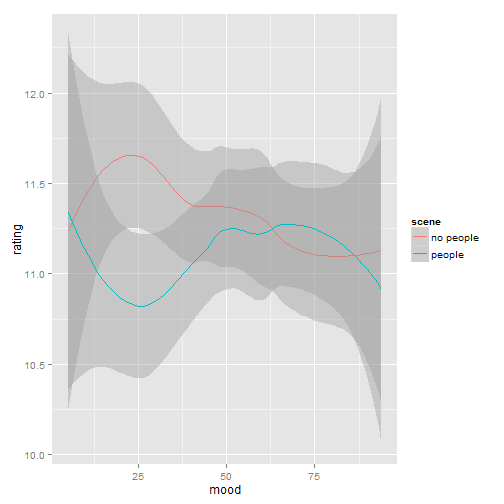
\includegraphics{Class6-figure/unnamed-chunk-42.png}
\caption{plot of chunk unnamed-chunk-42}
\end{figure}

\section{Plotting the interaction
(2)}\label{plotting-the-interaction-2-1}

\begin{itemize}
\itemsep1pt\parskip0pt\parsep0pt
\item
  Looks like the student was right!
\item
  Also looks like the effect is not really completely linear

  \begin{itemize}
  \itemsep1pt\parskip0pt\parsep0pt
  \item
    Maybe this is due to the subject and item effects in the data?
  \item
    Let's find out!
  \end{itemize}
\end{itemize}

\section{Start with linear
regression}\label{start-with-linear-regression}

\begin{itemize}
\itemsep1pt\parskip0pt\parsep0pt
\item
  Let's check our contrasts for \texttt{scene}
\end{itemize}

\begin{Shaded}
\begin{Highlighting}[]
\KeywordTok{contrasts}\NormalTok{(scene_liking$scene)}
\end{Highlighting}
\end{Shaded}

\begin{verbatim}
          people
no people      0
people         1
\end{verbatim}

\begin{itemize}
\itemsep1pt\parskip0pt\parsep0pt
\item
  Are we happy with this?

  \begin{itemize}
  \itemsep1pt\parskip0pt\parsep0pt
  \item
    Sure -- we just have to be aware of the coding when we interpret the
    coefficients
  \end{itemize}
\end{itemize}

\section{Run the model}\label{run-the-model}

\begin{Shaded}
\begin{Highlighting}[]
\NormalTok{scene_lm <-}\StringTok{ }\KeywordTok{lm}\NormalTok{(}\DataTypeTok{data =} \NormalTok{scene_liking, rating ~}\StringTok{ }\NormalTok{mood *}\StringTok{ }\NormalTok{scene)}
\KeywordTok{kable}\NormalTok{(}\KeywordTok{coef}\NormalTok{(}\KeywordTok{summary}\NormalTok{(scene_lm)))}
\end{Highlighting}
\end{Shaded}

\textbar{} \textbar{} Estimate\textbar{} Std. Error\textbar{} t
value\textbar{} Pr(\textgreater{}\textbar{}t\textbar{})\textbar{}
\textbar{}:----------------\textbar{}--------:\textbar{}----------:\textbar{}-------:\textbar{}------------------:\textbar{}
\textbar{}(Intercept) \textbar{} 11.7066\textbar{} 0.2475\textbar{}
47.2936\textbar{} 0.0000\textbar{} \textbar{}mood \textbar{}
-0.0073\textbar{} 0.0044\textbar{} -1.6505\textbar{} 0.0990\textbar{}
\textbar{}scenepeople \textbar{} -0.7583\textbar{} 0.3501\textbar{}
-2.1663\textbar{} 0.0304\textbar{} \textbar{}mood:scenepeople \textbar{}
0.0107\textbar{} 0.0063\textbar{} 1.6959\textbar{} 0.0901\textbar{} -
Where did the interaction go? - Let's do some quick diagnostics

\section{Regression diagnostics}\label{regression-diagnostics}

\begin{itemize}
\itemsep1pt\parskip0pt\parsep0pt
\item
  Multicollinearity?
\end{itemize}

\begin{Shaded}
\begin{Highlighting}[]
\KeywordTok{vif}\NormalTok{(scene_lm)}
\end{Highlighting}
\end{Shaded}

\begin{verbatim}
      mood      scene mood:scene 
      2.00       7.03       8.03 
\end{verbatim}

\begin{itemize}
\itemsep1pt\parskip0pt\parsep0pt
\item
  Aha! Those VIFs are quite a bit larger than 1. That spells trouble.
\item
  What is wrong?
\end{itemize}

\section{Addressing
multicollinearity}\label{addressing-multicollinearity}

\begin{itemize}
\itemsep1pt\parskip0pt\parsep0pt
\item
  What is wrong?
\item
  We forgot to center the continuous predictor \texttt{mood}
\item
  Let's fix this:
\end{itemize}

\begin{Shaded}
\begin{Highlighting}[]
\NormalTok{scene_liking$mood <-}\StringTok{ }\KeywordTok{scale}\NormalTok{(scene_liking$mood, }\DataTypeTok{scale =} \OtherTok{FALSE}\NormalTok{) }\CommentTok{# See Class 5}
\end{Highlighting}
\end{Shaded}

\section{Run the model again}\label{run-the-model-again}

\begin{Shaded}
\begin{Highlighting}[]
\NormalTok{scene_lm <-}\StringTok{ }\KeywordTok{lm}\NormalTok{(}\DataTypeTok{data =} \NormalTok{scene_liking, rating ~}\StringTok{ }\NormalTok{mood *}\StringTok{ }\NormalTok{scene)}
\KeywordTok{kable}\NormalTok{(}\KeywordTok{coef}\NormalTok{(}\KeywordTok{summary}\NormalTok{(scene_lm)))}
\end{Highlighting}
\end{Shaded}

\textbar{} \textbar{} Estimate\textbar{} Std. Error\textbar{} t
value\textbar{} Pr(\textgreater{}\textbar{}t\textbar{})\textbar{}
\textbar{}:----------------\textbar{}--------:\textbar{}----------:\textbar{}--------:\textbar{}------------------:\textbar{}
\textbar{}(Intercept) \textbar{} 11.3283\textbar{} 0.0934\textbar{}
121.3420\textbar{} 0.0000\textbar{} \textbar{}mood \textbar{}
-0.0073\textbar{} 0.0044\textbar{} -1.6505\textbar{} 0.0990\textbar{}
\textbar{}scenepeople \textbar{} -0.2085\textbar{} 0.1320\textbar{}
-1.5792\textbar{} 0.1145\textbar{} \textbar{}mood:scenepeople \textbar{}
0.0107\textbar{} 0.0063\textbar{} 1.6959\textbar{} 0.0901\textbar{} -
Still not quite there\ldots{} - Let's do more diagnostics

\section{Regression diagnostics --
again}\label{regression-diagnostics-again}

\begin{itemize}
\itemsep1pt\parskip0pt\parsep0pt
\item
  Multicollinearity?
\end{itemize}

\begin{Shaded}
\begin{Highlighting}[]
\KeywordTok{vif}\NormalTok{(scene_lm)}
\end{Highlighting}
\end{Shaded}

\begin{verbatim}
      mood      scene mood:scene 
         2          1          2 
\end{verbatim}

\begin{itemize}
\itemsep1pt\parskip0pt\parsep0pt
\item
  The VIFs are fine now.
\end{itemize}

\section{Influential cases}\label{influential-cases}

\begin{Shaded}
\begin{Highlighting}[]
\KeywordTok{kable}\NormalTok{(}\KeywordTok{head}\NormalTok{(}\KeywordTok{influence.measures}\NormalTok{(scene_lm)$infmat))}
\end{Highlighting}
\end{Shaded}

\textbar{} dfb.1\_\textbar{} dfb.mood\textbar{} dfb.scnp\textbar{}
dfb.md:s\textbar{} dffit\textbar{} cov.r\textbar{} cook.d\textbar{}
hat\textbar{}
\textbar{}-------:\textbar{}--------:\textbar{}--------:\textbar{}--------:\textbar{}-------:\textbar{}------:\textbar{}------:\textbar{}------:\textbar{}
\textbar{} 0.0000\textbar{} 0.0000\textbar{} 0.0101\textbar{}
0.0017\textbar{} 0.0145\textbar{} 1.0034\textbar{} 0.0001\textbar{}
0.0013\textbar{} \textbar{} -0.0376\textbar{} -0.0062\textbar{}
0.0266\textbar{} 0.0044\textbar{} -0.0381\textbar{} 1.0010\textbar{}
0.0004\textbar{} 0.0013\textbar{} \textbar{} 0.0000\textbar{}
0.0000\textbar{} -0.0041\textbar{} -0.0007\textbar{} -0.0059\textbar{}
1.0037\textbar{} 0.0000\textbar{} 0.0013\textbar{} \textbar{}
0.0093\textbar{} 0.0015\textbar{} -0.0066\textbar{} -0.0011\textbar{}
0.0095\textbar{} 1.0036\textbar{} 0.0000\textbar{} 0.0013\textbar{}
\textbar{} 0.0000\textbar{} 0.0000\textbar{} 0.0111\textbar{}
0.0018\textbar{} 0.0159\textbar{} 1.0033\textbar{} 0.0001\textbar{}
0.0013\textbar{} \textbar{} 0.0630\textbar{} 0.0104\textbar{}
-0.0446\textbar{} -0.0073\textbar{} 0.0639\textbar{} 0.9959\textbar{}
0.0010\textbar{} 0.0013\textbar{} - Any Cook's d greater than 1?

\begin{Shaded}
\begin{Highlighting}[]
\KeywordTok{sum}\NormalTok{(}\KeywordTok{cooks.distance}\NormalTok{(scene_lm) >}\StringTok{ }\DecValTok{1} \NormalTok{)}
\end{Highlighting}
\end{Shaded}

\begin{verbatim}
[1] 0
\end{verbatim}

\begin{itemize}
\itemsep1pt\parskip0pt\parsep0pt
\item
  Doesn't look like it, so we should be fine here.
\end{itemize}

\section{Normality}\label{normality}

\begin{Shaded}
\begin{Highlighting}[]
\KeywordTok{shapiro.test}\NormalTok{(}\KeywordTok{resid}\NormalTok{(scene_lm))}
\end{Highlighting}
\end{Shaded}

\begin{verbatim}

    Shapiro-Wilk normality test

data:  resid(scene_lm)
W = 0.9949, p-value = 2.632e-05
\end{verbatim}

\begin{itemize}
\itemsep1pt\parskip0pt\parsep0pt
\item
  Whoa! But we saw this in the plot already
\end{itemize}

\section{Q-Q Plots}\label{q-q-plots}

\begin{itemize}
\itemsep1pt\parskip0pt\parsep0pt
\item
  Here's a visual way to assess normality
\item
  Quantile-Quantile Plot: Split data into a number of quantiles and plot
  them against the quantiles of a hypothetical normal distribution
\end{itemize}

\begin{Shaded}
\begin{Highlighting}[]
\KeywordTok{qqnorm}\NormalTok{(}\KeywordTok{resid}\NormalTok{(scene_lm))}
\CommentTok{# if the distribution is normal, the points should be on this line}
\KeywordTok{qqline}\NormalTok{(}\KeywordTok{resid}\NormalTok{(scene_lm))}
\end{Highlighting}
\end{Shaded}

\begin{figure}[htbp]
\centering
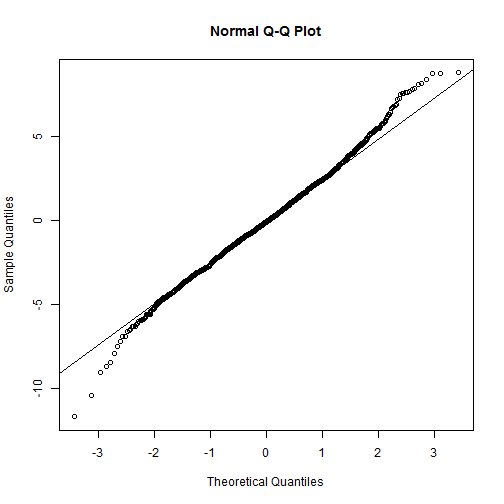
\includegraphics{Class6-figure/unnamed-chunk-52.png}
\caption{plot of chunk unnamed-chunk-52}
\end{figure}

\section{How to fix this?}\label{how-to-fix-this}

\begin{itemize}
\itemsep1pt\parskip0pt\parsep0pt
\item
  As a first step, remember that there are subject and item effects in
  these data
\item
  \texttt{lm} can't account for them, so we need something more powerful
\item
  Linear Mixed Models!
\item
  We use the function \texttt{lmer} (``Linear mixed effects
  regression'') from the \texttt{lme4} package
\item
  If you don't have \texttt{lme4} yet, install it by typing
  \texttt{install.packages("lme4")} in the Console
\end{itemize}

\section{Adding random subject and item
effects}\label{adding-random-subject-and-item-effects}

\begin{itemize}
\itemsep1pt\parskip0pt\parsep0pt
\item
  As a first step, we want our model to allow subjects and items to have
  different intercepts

  \begin{itemize}
  \itemsep1pt\parskip0pt\parsep0pt
  \item
    For example, Subject 1 might just really dislike the whole
    experiment and rate all scenes lower
  \item
    Or Item 33 might be particularly ugly and be disliked by all
    subjects
  \end{itemize}
\item
  Formally, our model will look like this:
  $y_{ij} = \beta_0 + \beta_1 x_{1} + \beta_2 x_{2} + \gamma_{0i} + \gamma_{0j} + \epsilon_{ij}$,
  where $y_{ij}$ is the response of subject $i$ to item $j$,
  $\gamma_{0i}$ is the intercept for subject $i$ and $\gamma_{0j}$ is
  the intercept for item $j$
\end{itemize}

\section{Running the model}\label{running-the-model}

\begin{itemize}
\itemsep1pt\parskip0pt\parsep0pt
\item
  In \texttt{lmer}, we specify the model in a formula just like in
  \texttt{lm}, but we add random effects terms, e.g.
  \texttt{(1\textbar{}subject)}

  \begin{itemize}
  \itemsep1pt\parskip0pt\parsep0pt
  \item
    The left side of the pipe stands for the random effect, the right
    side stands for the group for which we want to define the random
    effect
  \item
    \texttt{1} stands for the intercept. It is implicitly added,
    \emph{except} when there is no other predictor
  \end{itemize}
\end{itemize}

\begin{Shaded}
\begin{Highlighting}[]
\KeywordTok{library}\NormalTok{(lme4)}
\NormalTok{scene_lmm <-}\StringTok{ }\KeywordTok{lmer}\NormalTok{(}\DataTypeTok{data =} \NormalTok{scene_liking, rating ~}\StringTok{ }\NormalTok{scene *}\StringTok{ }\NormalTok{mood +}\StringTok{ }\NormalTok{(}\DecValTok{1}\NormalTok{|subject) +}\StringTok{ }\NormalTok{(}\DecValTok{1}\NormalTok{|item))}
\end{Highlighting}
\end{Shaded}

\section{Examining the model}\label{examining-the-model}

\begin{Shaded}
\begin{Highlighting}[]
\KeywordTok{summary}\NormalTok{(scene_lmm)}
\end{Highlighting}
\end{Shaded}

\begin{verbatim}
Linear mixed model fit by REML ['lmerMod']
Formula: rating ~ scene * mood + (1 | subject) + (1 | item)
   Data: scene_liking

REML criterion at convergence: 7657

Scaled residuals: 
   Min     1Q Median     3Q    Max 
-4.378 -0.617 -0.029  0.638  3.541 

Random effects:
 Groups   Name        Variance Std.Dev.
 subject  (Intercept) 0.0872   0.295   
 item     (Intercept) 0.1310   0.362   
 Residual             6.7615   2.600   
Number of obs: 1600, groups:  subject, 40; item, 40

Fixed effects:
                 Estimate Std. Error t value
(Intercept)      11.32825    0.11793    96.1
scenepeople      -0.20850    0.13001    -1.6
mood             -0.00755    0.00492    -1.5
scenepeople:mood  0.01108    0.00623     1.8

Correlation of Fixed Effects:
            (Intr) scnppl mood  
scenepeople -0.551              
mood         0.000  0.000       
sceneppl:md  0.000  0.000 -0.632
\end{verbatim}

\section{Understanding the model
output}\label{understanding-the-model-output}

\begin{itemize}
\itemsep1pt\parskip0pt\parsep0pt
\item
  Just like in logistic regression, LMMs are fitted in an iterative
  procedure using Maximum Likelihood (ML)

  \begin{itemize}
  \itemsep1pt\parskip0pt\parsep0pt
  \item
    Actually, \texttt{lmer} uses a slightly modified criterion called
    Restricted Maximum Likelihood (REML)
  \end{itemize}
\item
  Residuals can be interpreted just like in a regular linear model
\item
  Random effects: Here we get an estimate of the variance (and standard
  deviation) explained by the random intercepts

  \begin{itemize}
  \itemsep1pt\parskip0pt\parsep0pt
  \item
    We also get an estimate of the residual variance
  \end{itemize}
\item
  Check the number of observations to see if there are any missing that
  shouldn't be missing
\end{itemize}

\section{Coefficients}\label{coefficients}

\begin{Shaded}
\begin{Highlighting}[]
\KeywordTok{kable}\NormalTok{(}\KeywordTok{coef}\NormalTok{(}\KeywordTok{summary}\NormalTok{(scene_lmm)))}
\end{Highlighting}
\end{Shaded}

\textbar{} \textbar{} Estimate\textbar{} Std. Error\textbar{} t
value\textbar{}
\textbar{}:----------------\textbar{}--------:\textbar{}----------:\textbar{}-------:\textbar{}
\textbar{}(Intercept) \textbar{} 11.3283\textbar{} 0.1179\textbar{}
96.0573\textbar{} \textbar{}scenepeople \textbar{} -0.2085\textbar{}
0.1300\textbar{} -1.6037\textbar{} \textbar{}mood \textbar{}
-0.0075\textbar{} 0.0049\textbar{} -1.5336\textbar{}
\textbar{}scenepeople:mood \textbar{} 0.0111\textbar{} 0.0062\textbar{}
1.7801\textbar{} - First thing you notice: There's no p value! - That's
because, due to the shrinkage procedure, it isn't clear what the df of
that \emph{t}-value should be - In general, if the number of subjects is
\textgreater{} 30, we should be able to interpret the \emph{t} value
like a \emph{z} value, meaning that any \emph{t} \textgreater{} 2 or
\textless{} -2 should be significant

\section{Correlation of fixed
effects}\label{correlation-of-fixed-effects}

\begin{itemize}
\itemsep1pt\parskip0pt\parsep0pt
\item
  These are the estimated correlations of the fixed effects

  \begin{itemize}
  \itemsep1pt\parskip0pt\parsep0pt
  \item
    If any of these is \textgreater{} .8, you're in multicollinearity
    trouble!
  \end{itemize}
\end{itemize}

\section{Model comparisons}\label{model-comparisons-1}

\begin{itemize}
\itemsep1pt\parskip0pt\parsep0pt
\item
  Unfortunately, F-tests won't work, because we don't know what the
  $df_{Error}$ would be
\item
  But we can do the likelihood ratio test (LRT)
\item
  As always, we use \texttt{Anova} from \texttt{car}. This one gives us
  \emph{p} values!
\end{itemize}

\begin{Shaded}
\begin{Highlighting}[]
\KeywordTok{library}\NormalTok{(car)}
\KeywordTok{Anova}\NormalTok{(scene_lmm)}
\end{Highlighting}
\end{Shaded}

\begin{verbatim}
Analysis of Deviance Table (Type II Wald chisquare tests)

Response: rating
           Chisq Df Pr(>Chisq)  
scene       2.57  1      0.109  
mood        0.28  1      0.599  
scene:mood  3.17  1      0.075 .
---
Signif. codes:  0 '***' 0.001 '**' 0.01 '*' 0.05 '.' 0.1 ' ' 1
\end{verbatim}

\section{More model diagnostics}\label{more-model-diagnostics}

\begin{itemize}
\itemsep1pt\parskip0pt\parsep0pt
\item
  Something still seems to be wrong with this model. How about testing
  the normality assumption again?
\end{itemize}

\begin{Shaded}
\begin{Highlighting}[]
\KeywordTok{shapiro.test}\NormalTok{(}\KeywordTok{resid}\NormalTok{(scene_lmm))}
\end{Highlighting}
\end{Shaded}

\begin{verbatim}

    Shapiro-Wilk normality test

data:  resid(scene_lmm)
W = 0.9939, p-value = 3.583e-06
\end{verbatim}

\begin{itemize}
\itemsep1pt\parskip0pt\parsep0pt
\item
  Still significant? Maybe there still is a random effect that we
  haven't accounted for.
\end{itemize}

\section{Random slopes}\label{random-slopes}

\begin{itemize}
\itemsep1pt\parskip0pt\parsep0pt
\item
  We can also allow the regression slopes to vary by subject or item.
\item
  What are possible random slopes that we could consider?

  \begin{itemize}
  \itemsep1pt\parskip0pt\parsep0pt
  \item
    Important: in theory, you could add random slopes for all fixed
    effects, but in practice, your data might not have enough
    information to fit these
  \item
    In this case, there simply isn't enough data to fit random slopes
    for the interaction

    \begin{itemize}
    \itemsep1pt\parskip0pt\parsep0pt
    \item
      How do you know this?

      \begin{itemize}
      \itemsep1pt\parskip0pt\parsep0pt
      \item
        Well, your model will simply fail to converge if there is not
        enough data for a solution!
      \item
        Even if there \emph{is} enough data, multicollinearity can cause
        convergence failures, too.
      \end{itemize}
    \end{itemize}
  \item
    In our case, some reasonable random slopes would be \texttt{scene}
    for subjects (do some people react more strongly to scenes with
    people than others) and \texttt{mood} for items (are some items
    really hated by people in a bad mood?)
  \end{itemize}
\end{itemize}

\section{Random slopes (2)}\label{random-slopes-2}

\begin{itemize}
\itemsep1pt\parskip0pt\parsep0pt
\item
  If we include a random slope for subjects for $beta_1$, our model
  looks like this:
  $y_{ij} = \beta_0 + \beta_1 x_{1} + \beta_2 x_{2} + \gamma_{0i} + \gamma_{1i} x_{1} + \gamma_{0j} + \epsilon_{ij}$
\item
  We can tell \texttt{lmer} to fit such models like this (note that the
  intercept is implicit again in \texttt{(mood\textbar{}item)} and
  `(scene\textbar{}subject).

  \begin{itemize}
  \itemsep1pt\parskip0pt\parsep0pt
  \item
    Note that we don't have enough data to include both random effects
    in one model.
  \end{itemize}
\end{itemize}

\begin{Shaded}
\begin{Highlighting}[]
\NormalTok{scene_lmm_mood <-}\StringTok{ }\KeywordTok{lmer}\NormalTok{(}\DataTypeTok{data =} \NormalTok{scene_liking, rating ~}\StringTok{ }\NormalTok{scene *}\StringTok{ }\NormalTok{mood +}\StringTok{ }\NormalTok{(}\DecValTok{1}\NormalTok{|subject) +}\StringTok{ }\NormalTok{(mood|item))}
\NormalTok{scene_lmm_scene <-}\StringTok{ }\KeywordTok{lmer}\NormalTok{(}\DataTypeTok{data =} \NormalTok{scene_liking, rating ~}\StringTok{ }\NormalTok{scene *}\StringTok{ }\NormalTok{mood +}\StringTok{ }\NormalTok{(scene|subject) +}\StringTok{ }\NormalTok{(}\DecValTok{1}\NormalTok{|item))}
\end{Highlighting}
\end{Shaded}

\section{Testing the effect of random
slopes}\label{testing-the-effect-of-random-slopes}

\begin{itemize}
\itemsep1pt\parskip0pt\parsep0pt
\item
  We can use the LRT to test whether the slopes actually improve the
  models.

  \begin{itemize}
  \itemsep1pt\parskip0pt\parsep0pt
  \item
    We use the \texttt{anova} command (lower case \texttt{a}) to compare
    each random slope model with the random intercept model we fitted
    earlier
  \end{itemize}
\end{itemize}

\begin{Shaded}
\begin{Highlighting}[]
\KeywordTok{anova}\NormalTok{(scene_lmm, scene_lmm_mood)}
\end{Highlighting}
\end{Shaded}

\begin{verbatim}
Data: scene_liking
Models:
scene_lmm: rating ~ scene * mood + (1 | subject) + (1 | item)
scene_lmm_mood: rating ~ scene * mood + (1 | subject) + (mood | item)
               Df  AIC  BIC logLik deviance Chisq Chi Df Pr(>Chisq)    
scene_lmm       7 7648 7686  -3817     7634                            
scene_lmm_mood  9 6891 6939  -3436     6873   761      2     <2e-16 ***
---
Signif. codes:  0 '***' 0.001 '**' 0.01 '*' 0.05 '.' 0.1 ' ' 1
\end{verbatim}

\begin{itemize}
\itemsep1pt\parskip0pt\parsep0pt
\item
  Seems to improve the model! (Note that R automatically uses ML instead
  of REML for model comparison)
\end{itemize}

\section{Testing the effect of random
slopes}\label{testing-the-effect-of-random-slopes-1}

\begin{Shaded}
\begin{Highlighting}[]
\KeywordTok{anova}\NormalTok{(scene_lmm, scene_lmm_scene)}
\end{Highlighting}
\end{Shaded}

\begin{verbatim}
Data: scene_liking
Models:
scene_lmm: rating ~ scene * mood + (1 | subject) + (1 | item)
scene_lmm_scene: rating ~ scene * mood + (scene | subject) + (1 | item)
                Df  AIC  BIC logLik deviance Chisq Chi Df Pr(>Chisq)
scene_lmm        7 7648 7686  -3817     7634                        
scene_lmm_scene  9 7652 7700  -3817     7634     0      2          1
\end{verbatim}

\begin{itemize}
\itemsep1pt\parskip0pt\parsep0pt
\item
  No improvement here.
\end{itemize}

\section{Diagnostics -- yet again!}\label{diagnostics-yet-again}

\begin{Shaded}
\begin{Highlighting}[]
\KeywordTok{shapiro.test}\NormalTok{(}\KeywordTok{resid}\NormalTok{(scene_lmm_mood))}
\end{Highlighting}
\end{Shaded}

\begin{verbatim}

    Shapiro-Wilk normality test

data:  resid(scene_lmm_mood)
W = 0.9982, p-value = 0.07537
\end{verbatim}

\begin{itemize}
\itemsep1pt\parskip0pt\parsep0pt
\item
  Looks like adding a random slope for \texttt{mood} also (mostly) fixed
  our normality problem
\end{itemize}

\section{Interpreting the
coefficients}\label{interpreting-the-coefficients}

\begin{Shaded}
\begin{Highlighting}[]
\KeywordTok{kable}\NormalTok{(}\KeywordTok{coef}\NormalTok{(}\KeywordTok{summary}\NormalTok{(scene_lmm_mood)))}
\end{Highlighting}
\end{Shaded}

\textbar{} \textbar{} Estimate\textbar{} Std. Error\textbar{} t
value\textbar{}
\textbar{}:----------------\textbar{}--------:\textbar{}----------:\textbar{}-------:\textbar{}
\textbar{}(Intercept) \textbar{} 11.3554\textbar{} 0.1181\textbar{}
96.1116\textbar{} \textbar{}scenepeople \textbar{} -0.2628\textbar{}
0.0979\textbar{} -2.6836\textbar{} \textbar{}mood \textbar{}
-0.0070\textbar{} 0.0137\textbar{} -0.5148\textbar{}
\textbar{}scenepeople:mood \textbar{} 0.0101\textbar{} 0.0047\textbar{}
2.1568\textbar{} - Now we have significant effects! - Remember that
scene was coded as 0 = no people, 1 = people - Looks like, on average,
subjects gave the scene a rating that was -.26 lower when it contained
people than when it didn't. - The interaction is also significant. When
the scene contained no people, there was a very weak, non-significant
negative effect of mood. - When the scene did contain people, there was
a significant change in the effect of mood (with each point on the mood
scale increasing the picture rating by -.007 + .0101 = .0031). Not a
huge effect, but significant.

\section{Writing it up}\label{writing-it-up}

\begin{itemize}
\itemsep1pt\parskip0pt\parsep0pt
\item
  See the exercise!
\end{itemize}

\section{Thank you!}\label{thank-you}

\begin{itemize}
\itemsep1pt\parskip0pt\parsep0pt
\item
  I know this was (and still is) a massive effort
\item
  Thank you for staying motivated and engaging with the material.
\item
  As always, come see me if you have questions!
\end{itemize}

\end{document}
